\documentclass{jknotes}
\usepackage{joshkirklin}

\begin{document}

\institution{Cambridge Part III Maths}
\title{Applications of Differential Geometry to Physics}
\lecturer{Maciej Dunajski}
\notetaker{Josh Kirklin}
\date{Lent 2016}

\maketitle
\suggestionsspiel
\tableofcontents

\section{Introduction}
\lecture{14/01/16}
Geometry has always played a key role in physics. For example, consider Kepler orbits, i.e. paths \(\vb{r}(t)\) in \(\RR^3\) obeying:
\begin{equation}
    \dot{\vb{r}} = \frac{GM}{r^3}\vb{r}
\end{equation}

\begin{wrapfigure}{l}{0.3\linewidth}
    \centering
    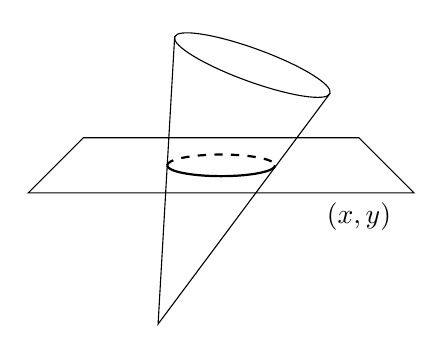
\begin{tikzpicture}[scale=0.7]
        \node[below] at (6,0) {\((x,y)\)};
        \draw (0,0) -- (1,1) -- (6,1) -- (7,0) -- cycle;
        \begin{scope}[shift={(3.5,0.5)},yscale=0.2,thick]
            \draw (-0.98,0) arc (-180:0:0.98);
            \draw[dashed] (-0.98,0) arc (180:0:0.98);
        \end{scope}
        \begin{scope}[shift={(3.04,-0.5)}, rotate=-20]
            \draw (-1.5,3) -- (0,-2) -- (1.5,3);
            \draw (0,3) ellipse (1.5 and 0.3);
        \end{scope}
    \end{tikzpicture}
\end{wrapfigure}
The solutions are conic sections. If we view a conic section as a path with coordinates \((x,y)\) in the plane it inhabits, then we can find that all conic sections can be written as the locus of solutions of an equation of the following form:
\begin{equation}
    ay^2 +  bx^2 + cxy + dy + ex + f = 0
\end{equation}
where \(a,b,c,d,e,f \in\RR\). It was first deduced by Apollonius of Perga that given five arbitrary points in the plane, there is a unique conic section through those points. Thus if we observe the position of a planet at five different points, we can deduce its orbit.

The space of conic sections is \(\mathbb{RP}^5=\RR^6/\sim\) where \(x\sim y \iff \Exists C \in \RR \st x = Cy\). We can see this by first labelling each conic section by its coefficients \((a,b,c,d,e,f)\in \RR^6\) in the above equation, and then seeing that we can simply multiply both sides of the equation to get the same conic.

This is geometry, but it is an algebraic sort of geometry. In this course we will be more interested in \emph{differential} geometry. There will be three main topics that we will cover in some detail:
\begin{description}
    \item[The Hamiltonian formalism] (19th century), which involves a generalised coordinate \(q\), its conjugate momentum \(p\), and a function \(H(p,q)\) such that paths in \((p,q)\) space obey:
        \begin{equation}
            \dot{q}=\pdv{H}{p},\quad\dot{p}=-\pdv{H}{q}
        \end{equation}
        We will see how this leads to a notion of \emph{symplectic geometry} (20th century), which concerns \emph{symplectomorphisms}, which are diffeomorphisms that preserve \(\int\dd{p}\wedge\dd{q}\), and are generated by Hamiltonian vector fields: \(X_H=\pdv{H}{p}\pdv{q}-\pdv{H}{q}\pdv{p}\).
    \item[General relativity] (1915), which leads to \emph{Riemannian geometry}.
    \item[Gauge theory] (both Maxwell and Yang-Mills), which will lead to discussions on an object known as the connection on a \emph{principal bundle}.
\end{description}

A unifying feature of these topics will be the presence of Lie groups.

This course will involve lots of examples (often instead of proofs), and the emphasis will be on calculations.

\subsection{Manifolds}
\begin{defn}
    An \(n\)-dimensional (smooth) \emph{manifold} is a set \(\mathcal{M}\) together with a collection of open sets \(U_\alpha\), \(\alpha = 1,2,\dots\), such that the \(U_\alpha\) cover \(\mathcal{M}\), and there exist bijections \(\phi_\alpha:U_\alpha\rightarrow V_\alpha\subset\RR^n\) (called \emph{charts}) such that \(\phi_\beta\circ\phi_\alpha^{-1}:\phi_\alpha(U_\alpha\cap U_\beta) \rightarrow \phi_\beta(U_\alpha\cap U_\beta)\) is smooth.
\end{defn}

\begin{figure}[H]
    \centering
    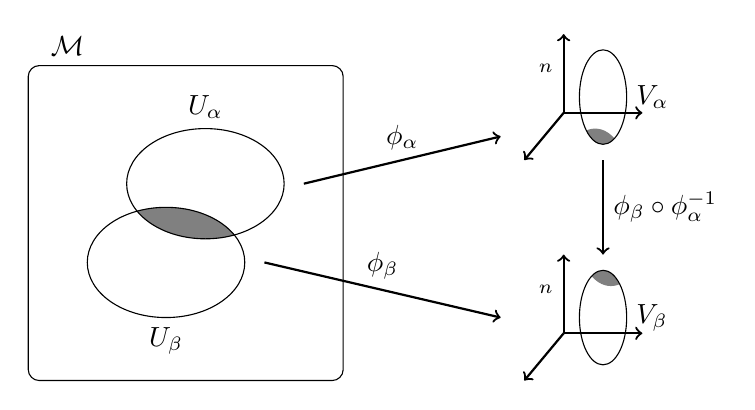
\begin{tikzpicture}
        \node[above] at (0.5,4) {\(\mathcal{M}\)};
        \draw[rounded corners] (0,0) rectangle (4,4);
        \begin{scope}
            \clip (1.75,1.5) ellipse (1 and 0.7);
            \fill[gray] (2.25,2.5) ellipse (1 and 0.7);
        \end{scope}
        \draw (1.75,1.5) ellipse (1 and 0.7);
        \draw (2.25,2.5) ellipse (1 and 0.7);
        \node[below] at (1.75,0.8) {\(U_\beta\)};
        \node[above] at (2.25,3.2) {\(U_\alpha\)};
        
        \begin{scope}[shift={(6.8,0.6)}]
            \draw[thick,->] (0,0) -- (1,0);
            \draw[thick,->] (0,0) -- (0,1);
            \draw[thick,->] (0,0) -- (-0.5,-0.6);
            \begin{scope}
                \clip (0.5,0.2) ellipse (0.3 and 0.6);
                \fill[gray] (0.6,1.2) ellipse (0.4 and 0.6);
            \end{scope}
            \draw (0.5,0.2) ellipse (0.3 and 0.6);
            \node[right] at (0.8,0.2) {\(V_\beta\)};
            \node[left] at (0,0.5) {\(\RR^n\)};
        \end{scope}
        
        \begin{scope}[shift={(6.8,3.4)}]
            \draw[thick,->] (0,0) -- (1,0);
            \draw[thick,->] (0,0) -- (0,1);
            \draw[thick,->] (0,0) -- (-0.5,-0.6);
            \begin{scope}
                \clip (0.5,0.2) ellipse (0.3 and 0.6);
                \fill[gray] (0.4,-0.8) ellipse (0.4 and 0.6);
            \end{scope}
            \draw (0.5,0.2) ellipse (0.3 and 0.6);
            \node[right] at (0.8,0.2) {\(V_\alpha\)};
            \node[left] at (0,0.5) {\(\RR^n\)};
        \end{scope}

        \draw[thick,->] (3.5,2.5) -- (6,3.1) node[midway,above] {\(\phi_\alpha\)};
        \draw[thick,->] (3,1.5) -- (6,0.8) node[midway,above] {\(\phi_\beta\)};
        \draw[thick,->] (7.3,2.8) -- (7.3,1.6) node[midway,right] {\(\phi_\beta\circ\phi_\alpha^{-1}\)};
    \end{tikzpicture}
\end{figure}
Informally, we can say that \(M\) is a topological space with some extra structure that allows us to introduce a differential calculus.

\begin{eg}
    The trivial manifold is \(\mathcal{M} = \RR^n\) with a single chart, for example the identity.
\end{eg}
Although it is not obvious, it is in fact usually possible to choose other differential structures on \(\RR^n\). For example, it has been shown that there are infinitely many \emph{exotic structures} on \(\RR^4\) (Donaldson 1984).
\begin{eg}
    The \(n\)-dimensional sphere \(S^n=\{\vb{r}\in\RR^{n+1}\st |\vb{r}|=1\}\subset \RR^{n+1}\) is an \(n\)-manifold. We choose open sets \(U = S^n \setminus N, \tilde{U} = S^n \setminus S\) where \(N = \{0,\dots,0,1\}\), \(S = \{0,\dots,0,-1\}\), and define charts as follows:
    \begin{figure}[H]
        \centering
        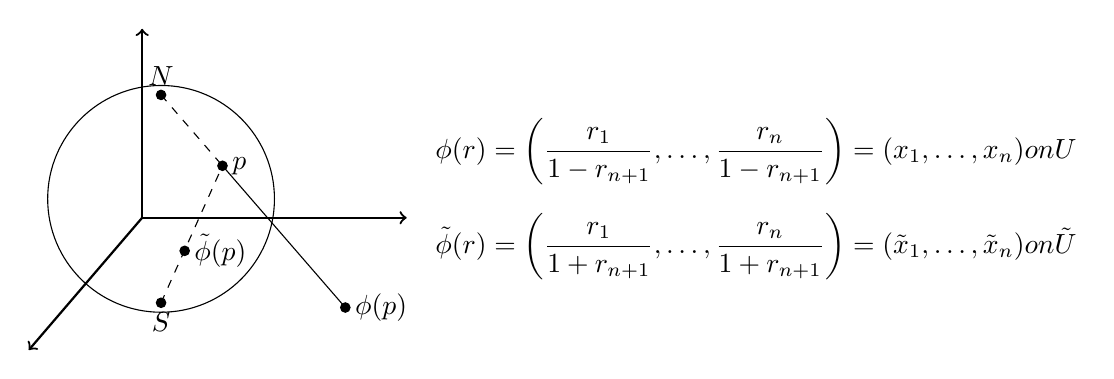
\begin{tikzpicture}[scale=1.2]
            \draw[thick,->] (0,0) -- (2.8,0);
            \draw[thick,->] (0,0) -- (0,2);
            \draw[thick,->] (0,0) -- (-1.2,-1.4);
            \draw (0.2,0.2) circle (1.2);
            
            \draw[dashed] (0.2,1.3) -- (0.85,0.55);
            \draw (0.85,0.55) -- (2.15,-0.95);
            \draw[fill] (2.15,-0.95) circle (0.05) node[right] {\(\phi(p)\)};

            \draw[dashed] (0.2,-0.9) -- (0.85,0.55);
            \draw[fill] (0.45,-0.35) circle (0.05) node[right] {\(\tilde\phi(p)\)};

            \draw[fill] (0.85,0.55) circle (0.05) node[right] {\(p\)};
            \draw[fill] (0.2,1.3) circle (0.05) node[above] {\(N\)};
            \draw[fill] (0.2,-0.9) circle (0.05) node[below] {\(S\)};

            \node[right] at (3,0.7) {\(\displaystyle
                \phi(\vb{r}) = \left( \frac{r_1}{1-r_{n+1}},\dots,\frac{r_n}{1-r_{n+1}} \right) = (x_1,\dots,x_n) \text{ on } U
            \)};
            \node[right] at (3,-0.3) {\(\displaystyle
                \tilde\phi(\vb{r}) = \left( \frac{r_1}{1+r_{n+1}},\dots,\frac{r_n}{1+r_{n+1}} \right) = (\tilde{x}_1,\dots,\tilde{x}_n) \text{ on } \tilde{U}
            \)};
        \end{tikzpicture}
    \end{figure}
    Note that:
    \begin{equation}
        x_1^2+\dots+x_n^2 = \frac{r_1^2+\dots+r_n^2}{(1-r_{n+1})^2} = \frac{1 - r_{n+1}^2}{(1-r_{n+1})^2} = \frac{1 + r_{n+1}}{1-r_{n+1}}
    \end{equation}
    So:
    \begin{equation}
        \tilde{x}_k = \frac{1-r_{n+1}}{1+r_{n+1}} x_k = \frac{x_k}{x_1^2+\dots+x_n^2}
    \end{equation}
    is smooth on \(U\cap \tilde{U}\).
\end{eg}

\begin{eg}
    Let \(f_1,\dots,f_k:\RR^N\rightarrow\RR\) and set \(M = \{\vb{r}\in\RR^N\st f_1 = \dots = f_k = 0\}\). Then \(M\) is a manifold if \(\rank\pdv{f^i}{x^a}\) is maximal, and is called a \emph{surface} in \(\RR^N\).
\end{eg}
In fact:
\begin{theorem}[Whitney]
    Any \(n\)-dimensional manifold \(\mathcal{M}\) can be obtained as a surface in \(\RR^N\), where \(N \le 2n+1\).
\end{theorem}
\begin{eg}
    Real projective space \(\mathbb{RP^n}\) is a manifold:
    \begin{equation}
        \mathbb{RP}^n = \frac{\RR^{n+1}\setminus{0}}{\sim} \qq{where} [X^1,\dots,X^{n+1}] \sim [cX^1,\dots,xC^{n+1}] \qq{for all} c \in \RR^* = \RR \setminus {0}
    \end{equation}
    We have \(n+1\) open sets \(U_\alpha = \{p\in\mathbb{RP}^n\st X^\alpha \ne 0\}\), and charts on each open set:
    \begin{equation}
        x_1 = \frac{X^1}{X^\alpha},\quad\dots\quad x_{\alpha-1} = \frac{X^{\alpha-1}}{X^\alpha},\quad x_{\alpha+1} = \frac{X^{\alpha+1}}{X^\alpha},\quad \dots\quad x_{n+1} = \frac{X^{n+1}}{X^\alpha}
    \end{equation}
\end{eg}

\subsection{Vector Fields}
\lecture{19/01/16}

Suppose we have two manifolds \(\mathcal{M},\tilde{\mathcal{M}}\) with dimensions \(n,\tilde{n}\), open sets \(U_\alpha,\tilde{U}_\beta\) and charts \(\phi_\alpha,\phi_\beta\) respectively, and let \(f\) be a map from \(\mathcal{M}\) to \(\tilde{\mathcal{M}}\).

\begin{defn}
    \(f\) is \emph{smooth} if \(\tilde{\phi}_\beta\circ f\circ\phi_\alpha^{-1}:\RR^n\rightarrow\RR^{\tilde{n}}\) is smooth for all \(\alpha, \beta\).
\end{defn}

\begin{defn}
    If \(\tilde{\mathcal{M}}=\RR\), then \(f:\mathcal{M}\rightarrow\RR\) is a \emph{function}.
\end{defn}

\begin{defn}
    If \(\mathcal{M} = \RR\), then \(f:\RR\rightarrow\tilde{\mathcal{M}}\) is a \emph{curve}.
\end{defn}

Suppose we have a curve \(\gamma:\RR\rightarrow\mathcal{M}\) such that \(\gamma(0) = p \in \mathcal{M}\). Let \(U\) be an open neighbourhood of \(p\), \(U\simeq\RR^n\) and choose coordinates \(x^a\), \(a = 1,\dots,n\) on \(U\).

\begin{defn}
    The \emph{tangent vector} to \(\gamma\) at \(p\) is defined as:
    \begin{equation}
        V|_p = \left.\dv{\gamma(\epsilon)}{\epsilon}\right|_{\epsilon=0}\in T_p\mathcal{M}
    \end{equation}
    where \(T_p\mathcal{M}\) is the \emph{tangent space} at \(p\), defined as the set of all tangent vectors to all curves at \(p\).
    \begin{figure}[H]
        \centering
        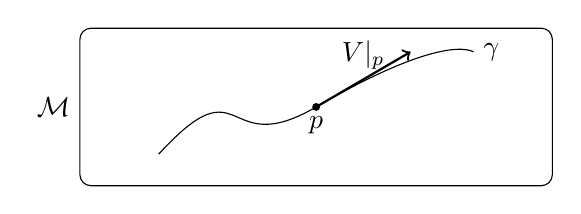
\begin{tikzpicture}
            \draw[rounded corners] (0,0) rectangle (6,2);
            \node[left] at (0,1) {\(\mathcal{M}\)};
            \draw (1,0.4) .. controls (2.1,1.6) and (1.8,0.3) .. (3,1)
                          .. controls (4.2,1.7) and (4.8,1.8) .. (5,1.7)
                          node[right] {\(\gamma\)};
            \fill (3,1) circle (0.05) node[below] {\(p\)};
            \draw[->, thick] (3,1) -- (4.2,1.7) node[midway,above] {\(V|_p\)};
        \end{tikzpicture}
    \end{figure}
\end{defn}

\begin{defn}
    The \emph{tangent bundle} is given by:
    \begin{equation}
        T\mathcal{M} = \bigcup_{\mathclap{p\in\mathcal{M}}} T_p\mathcal{M}
    \end{equation}
\end{defn}

A vector field assigns a tangent vector to each point \(p\in\mathcal{M}\). Let \(f:\mathcal{M}\rightarrow\RR\). The rate of change of \(f\) along \(\gamma\) is given by:
\begin{align}
    \dv{\epsilon}f(x^a(\epsilon))|_{\epsilon=0} &= \sum_{a=1}^n \dot{x}^a(\epsilon)\left.\pdv{f}{x^a}\right|_{\epsilon=0}\\
    &= \underbrace{\sum_{a=1}^nV^a(x)\left.\pdv{x^a}\right|_p}_{=V} f
\end{align}
\(V\) is a vector field. \(V^a(x)\) are the components of \(V\) in the basis \(\left\{\pdv{x^1},\dots,\pdv{x^n}\right\}\) at \(p\). 

We have gone from a curve to a vector field. We can also go the other way:
\begin{defn}
    An \emph{integral curve} or \emph{flow} \(\gamma(\epsilon)\) of a vector field \(V\) is defined by:
    \begin{equation}
        \dot{\gamma}(\epsilon) = V|_{\gamma(\epsilon)}
        \qq{or, equivalently}
        \dv{\epsilon}x^a(\epsilon) = V^a(x(\epsilon))
    \end{equation}
\end{defn}
We have:
\begin{equation}
    x^a(\epsilon,x^a(0)) = x^a(0) + \epsilon V^a(x(0)) + O(\epsilon^2)
\end{equation}
We say that the vector field \(V\) \emph{generates} the flow.
\begin{defn}
    An \emph{invariant} of a vector field \(V\) is a function that is constant along the flow of \(V\):
    \begin{equation}
        f(x^a(0)) = f(x^a(\epsilon)) \Forall \epsilon
        \qq{or, equivalently}
        V(f) = 0
    \end{equation}
\end{defn}
\begin{eg}
    Let \(\mathcal{M}=\RR^2\), \(x^a = (x,y)\), and \(V = x\pdv{x}+\pdv{y}\). The integral curves of \(V\) are given by \(\dot{x}=x\), \(\dot{y}=1\), and we can solve this to obtain \((x(\epsilon),y(\epsilon)) = (x(0)e^\epsilon,y(0)+\epsilon)\).
    \begin{figure}[H]
        \centering
        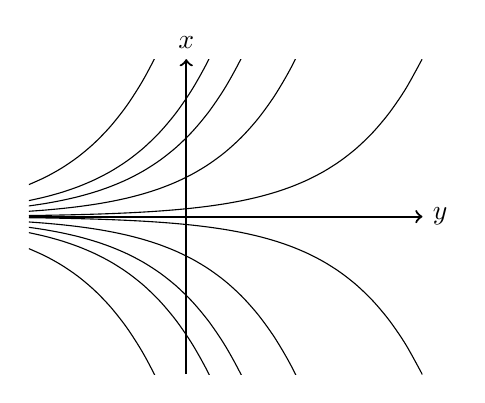
\begin{tikzpicture}
            \draw[thick,->] (-2,0) -- (3,0) node[right] {\(y\)};
            \draw[thick,->] (0,-2) -- (0,2) node[above] {\(x\)};
            \clip (-2,-2) rectangle (3,2);
            \draw[domain=-2:3,smooth,variable=\x] plot ({\x},{3*exp(\x)});
            \draw[domain=-2:3,smooth,variable=\x] plot ({\x},{1.5*exp(\x)});
            \draw[domain=-2:3,smooth,variable=\x] plot ({\x},{exp(\x)});
            \draw[domain=-2:3,smooth,variable=\x] plot ({\x},{0.5*exp(\x)});
            \draw[domain=-2:3,smooth,variable=\x] plot ({\x},{0.1*exp(\x)});
            \draw[domain=-2:3,smooth,variable=\x] plot ({\x},{-0.1*exp(\x)});
            \draw[domain=-2:3,smooth,variable=\x] plot ({\x},{-0.5*exp(\x)});
            \draw[domain=-2:3,smooth,variable=\x] plot ({\x},{-exp(\x)});
            \draw[domain=-2:3,smooth,variable=\x] plot ({\x},{-1.5*exp(\x)});
            \draw[domain=-2:3,smooth,variable=\x] plot ({\x},{-3*exp(\x)});
        \end{tikzpicture}
    \end{figure}
    Note that on these curves \(xe^{-y}\) is constant, so this is an invariant of \(V\).
\end{eg}
\begin{eg}
    Consider the 1-parameter group of rotations on \(\RR^2\). Under these rotations, \((x_0,y_0)\) transforms to the point \((x(\epsilon),y(\epsilon)) = (x_0\cos\epsilon-y_0\sin\epsilon,x_0\sin\epsilon+y_0\cos\epsilon)\). The vector field that generates these curves is given by:
    \begin{align}
        V &= \left( \dv{y(\epsilon)}{\epsilon}\pdv{y} + \dv{x(\epsilon)}{\epsilon}\pdv{\epsilon} \right)\\
        &= x\pdv{y} - y\pdv{x}
    \end{align}
    The distance to the origin is an invariant of \(V\):
    \begin{equation}
        V(x^2+y^2) = -2xy + 2xy = 0
    \end{equation}
\end{eg}
\begin{defn}
    A \emph{Lie bracket} of two vector fields \(V\) and \(W\) is a vector field \([V,W]\) defined by its action on functions as:
    \begin{equation}
        [V,W](f) = V(W(f))-W(V(f))
    \end{equation}
\end{defn}
The Lie bracket has some important properties:
\begin{description}
    \item[Antisymmetry]: \([V,W] = -[W,V]\)
    \item[Jacobi identity]: \([U,[V,W]] + [V,[W,U]] + [W,[U,V]] = 0\)
\end{description}
\begin{eg}
    If \(V = x\pdv{x}+\pdv{y}\) and \(W = \pdv{x}\), then \([V,W] = -\pdv{x} = -W\).
\end{eg}
\begin{defn}
    A \emph{Lie algebra} is a vector space \(\mathfrak{g}\) equipped with an antisymmetric bilinear operation \([\;,\;]:\mathfrak{g}\times\mathfrak{g}\rightarrow\mathfrak{g}\) that satisfies the Jacobi identity.
\end{defn}
If \(\mathfrak{g}\) is finite-dimensional and \(V_\alpha\), \(\alpha = 1,\dots,\dim\mathfrak{g}\) span \(\mathfrak{g}\), then \(\mathfrak{g}\) is determined by its structure constants \(f_{\alpha\beta}^\gamma\), defined as follows:
\begin{equation}
    [V_\alpha,V_\beta] = \sum_\gamma f_{\alpha\beta}^\gamma V_\gamma
\end{equation}
\begin{eg}
    There are only two 2D Lie algebras (up to isomorphism), each determined by the bracket of two basis elements:
    \begin{equation}
        [V,W] = 0 \qq{or} [V,W] = -W
    \end{equation}
\end{eg}
\begin{eg}
    \(gl(n,\RR)\) (the set of all \(n\times n\) real matrices) is a Lie algebra when equipped with the matrix commutator as a bracket. Its dimension is \(n^2\).
\end{eg}
\begin{eg}
    Vector fields on a manifold \(\mathcal{M}\) form an infinite dimensional Lie algebra. Consider for example \(\mathfrak{g} = \operatorname{diff}(S^1)\) or \(\operatorname{diff}(\RR)\), by which we mean the set of all vector fields on the manifold. We have the following basis of \(\mathfrak{g}\):
    \begin{equation}
        V_a = - x^{\alpha+1}\pdv{x} \qq{where} \alpha\in\ZZ
    \end{equation}
    With this basis, the Lie bracket gives:
    \begin{equation}
        [V_\alpha,V_\beta] = (\alpha-\beta)V_{\alpha+\beta}
    \end{equation}
\end{eg}

\lecture{21/01/16}
\begin{eg}
    The \emph{Virasoro algebra} is a so-called \emph{central extension} of \(\operatorname{diff}(S^1)\). This is defined as \(\text{Vir} = \operatorname{diff}(S^1) \oplus \RR\), and we choose \(c\in\RR\) to be a basis vector of the \(\RR\) sector (\(c\) is sometimes referred to as the \emph{central charge}). In addition, we have the following brackets:
    \begin{equation}
        [V_\alpha,c]_{\text{Vir}} = 0,\quad
        [V_\alpha,V_\beta]_{\text{Vir}} = (\alpha-\beta)V_{\alpha+\beta} + \frac{c}{12}(\alpha^3-\alpha)\delta_{\alpha+\beta,0}
    \end{equation}
    Consider the bracket of two vector fields in \(\operatorname{diff}(S^1)\):
    \begin{equation}
        \left[ f(x)\pdv{x},g(x)\pdv{x} \right] = (\underbrace{fg'-gf'}_{\text{Wronskian}}\pdv{x}
    \end{equation}
    This extends to the Virasoro algebra in a slightly non-trivial manner. According to Witten:
    \begin{equation}
        \left[ f(x)\pdv{x},g(x)\pdv{x} \right]_{\text{Vir}} = (fg'-gf')\pdv{x}
        + \frac{ic}{48\pi}\int(f_{xxx}g-g_{xxx}f)\dd{x}
    \end{equation}
\end{eg}
\begin{theorem}[Ado]
    Every finite-dimensional Lie algebra is isomorphic to some matrix algebra.
\end{theorem}

\section{Lie groups}
\begin{defn}
    A \emph{Lie group} is a group that is also a manifold such that the group operations \(G\times G\to G\), \((g_1,g_2)\to g_1g_2\) and \(G\to G\), \(g\to g^{-1}\) are smooth maps.
\end{defn}
\begin{eg}
    \(G=GL(n,\RR)\) is a Lie group with dimension \(n^2\).
\end{eg}
\begin{eg}
    \(G=O(n,\RR)\) is a Lie group with dimension \(\frac{n(n-1)}{2}\).
\end{eg}
\begin{defn}
    A \emph{group action} of a group \(G\) on a manifold \(\mathcal{M}\) is a function \(G\times\mathcal{M}\to\mathcal{M}\), \((g,p)\to g(p)\) such that \(e(p) = p\) and \(g_1(g_2(p)) = (g_1g_2)(p)\). Groups acting on manifolds are referred to as \emph{transformation groups}.
\end{defn}
\begin{eg}
    Consider \(\mathcal{M}=\RR^2\) and \(G=E(2)\), the 3-dimensional Euclidean group, consisting of rotations and translations of the plane. An element \(g \in G\) with coordinates \((\theta,a,b)\) acts on \(\mathcal{M}\) in the following way:
    \begin{equation}
        g
        \begin{pmatrix}
            x \\ y
        \end{pmatrix}
        = 
        \begin{pmatrix}
            \cos\theta & -\sin\theta \\
            \sin\theta & \cos\theta
        \end{pmatrix}
        \begin{pmatrix}
            x \\ y
        \end{pmatrix}
        +
        \begin{pmatrix}
            a \\ b
        \end{pmatrix}
    \end{equation}
    We see that the manifold of \(G\) is \(S^1\times \RR^2\). \(G\) has three 1-parameter Lie subgroups:
    \begin{itemize}
        \item \(G_\theta\), elements with coordinates \((\theta,0,0)\). 
        \item \(G_a\), elements with coordinates \((0,a,0)\). 
        \item \(G_b\), elements with coordinates \((0,0,b)\). 
    \end{itemize}
    Each 1-parameter subgroup with parameter \(\epsilon\) is in fact a flow, generated by the vector field:
    \begin{equation}
        V|_p = \left.\dv{\epsilon}\left( g_\epsilon(p) \right)\right|_{\epsilon=0}
    \end{equation}
    We have:
    \begin{equation}
        V_\theta = x\pdv{y}-y\pdv{x},\quad
        V_a = \pdv{x},\quad
        V_b = \pdv{y}
    \end{equation}
    These form a basis for a 3D Lie algebra of \(E(2)\), in which we have:
    \begin{equation}
        [V_a,V_\theta] = V_b,\quad
        [V_b,V_\theta] = -V_a,\quad
        [V_a,V_b] = 0
    \end{equation}
\end{eg}

\subsection{Geometry of Lie groups}
Let \(\mathcal{M}\) and \(\tilde{\mathcal{M}}\) be manifolds, and \(f:\mathcal{M}\to\tilde{\mathcal{M}}\).
\begin{defn}
    A tangent map \(f_*:T_p\mathcal{M}\to T_{f(p)}\tilde{\mathcal{M}}\) is defined by:
    \begin{equation}
        f_*(V) = \left.\dv{\epsilon} f(\gamma(\epsilon))\right|_{\epsilon=0}
    \end{equation}
    where \(\gamma\) is an integral curve of \(V\). This definition extends to \(T\mathcal{M}\)
    \begin{equation}
        (f_*(V))^i = V^j\pdv{f^i}{x^j}
    \end{equation}
    where \(i = 1,\dots,\dim\tilde{\mathcal{M}}\), \(j=1,\dots,\dim\mathcal{M}\).
\end{defn}
\begin{defn}
    Let \(V\), \(W\) be vector fields with \(V = \dot{\gamma}\). The \emph{Lie derivative} is defined as follows:
    \begin{equation}
        \mathcal{L}_VW = \lim_{\epsilon\to0} \frac{W(p) - \gamma(\epsilon)_*W(p(\epsilon))}{\epsilon} = [V,W]
    \end{equation}
    We also define \(\mathcal{L}_V(f) = V(f)\) for functions \(f\), and define Lie derivatives on higher order tensors by the Leibnitz rule.
\end{defn}

\lecture{26/01/16}
Given \(\Omega\) an \(r\)-form, we can find its Lie derivative using the Cartan formula:
\begin{equation}
    \mathcal{L}_V\Omega = \dd{V\contract\Omega} + V\contract\dd{\Omega}
\end{equation}

\begin{defn}
    A \emph{Lie algebra} \(\mathfrak{g}\) of a Lie group \(G\) is the tangent space of \(G\) at the identity, with bracket in \(\mathfrak{g}\) given by the commutator of fields on \(G\), defined in the following way. 
    Given a \(g\in G\), its associated left translation function is \(L_g:G\to G\), \(L_g(h) = gh\). This induces a map \((L_g)_*:\mathfrak{g}\to T_g(G)\). Given a \(v\in \mathfrak{g}\), the vector field \(g\mapsto(L_g)_*v\) is \emph{left-invariant}. The Lie bracket is then given in terms of commutators of these left-invariant fields:
    \begin{equation}
        [(L_g)_*v,(L_g)_*w] = (L_g)_*[v,w]_{\mathfrak{g}}
    \end{equation}
\end{defn}

If we have a basis of \(\mathfrak{g}\), then left translation naturally gives a set of \(\dim(G)\) independent global non-vanishing vector fields on \(\mathcal{G}\). Manifolds that admit such a set are said to be \emph{parallelisable}. (Note that not all parallelisable manifolds can be made into Lie groups.)

Let \(L_\alpha\), \(\alpha=1,\dots,\dim\mathfrak{g}\) be a basis of left invariant vector fields. The structure of the commutator is given by its structure constants
\begin{equation}
    [L_\alpha,L_\beta] = \sum_\gamma f^\gamma_{\alpha\beta} L_\gamma.
\end{equation}
Let \(\sigma^\alpha\) be a dual basis of left-invariant 1-forms, \(L_\alpha\contract\sigma^\beta = \delta^\beta_\alpha\). For any 1-form \(\Omega\) and vector fields \(v,w\), we have the identity
\begin{equation}
    \dd{\Omega}(v,w) = v(\Omega(w)) - w(\Omega(v)) - \Omega([v,w]),
\end{equation}
so in particular we have
\begin{equation}
    \dd{\sigma^\alpha} + \frac{1}{2}f^\alpha_{\beta\gamma}\sigma^\beta\wedge\sigma^\gamma = 0.
    \label{dualleft}
    \tag{\(*\)}
\end{equation}

\begin{defn}
    The \emph{Maurer-Cartan 1-form} \(\rho\) is a Lie algebra valued 1-form defined by \(\rho_g(v) = (L_{g^{-1}})_*v\).
\end{defn}
Assume from now on that \(G\) is a matrix Lie group, and let \(g \in G\). Then it can be shown that \(\rho_g=g^{-1}\dd{g}\). This is indeed left-invariant
\begin{equation}
    (g_0g)^{-1}\dd{(g_0g)} = g^{-1}g_0^{-1}g_0\dd{g} = g^{-1}\dd{g},
\end{equation}
and it is a member of the Lie algebra, as we can see by considering the curve
\begin{equation}
    g^{-1}(s)g(s+\epsilon) = e + \epsilon \underbrace{g^{-1}\left.\dv{g}{s}\right|_{\epsilon=0}}_{\in\mathfrak{g}} + O(\epsilon^2).
\end{equation}

We can expand the Maurer-Cartan 1-form as
\begin{equation}
    g^{-1}\dd{g} = \sum_\alpha\sigma^\alpha\otimes T_\alpha,
\end{equation}
where \(T_\alpha\) are matrices in a basis of \(\mathfrak{g}\) satisfying
\begin{equation}
    [T_\alpha,T_\beta] = \sum_\gamma f_{\alpha\beta}^\gamma T_\gamma.
\end{equation}

We have
\begin{equation}
    \dd{\rho} = \dd{g^{-1}}\wedge\dd{g} = -g^{-1}\dd{g}g^{-1}\wedge\dd{g} = -\rho\wedge\rho.
\end{equation}

\lecture{28/01/16}
In terms of the expansion,
\begin{equation}
    \dd{\sigma^\alpha}\otimes T_\alpha = \sigma^\alpha\wedge\sigma^\beta T_\alpha T_\beta = \frac{1}{2}\sigma^\alpha\wedge\sigma^\beta[T_\alpha,T_\beta] = \frac{1}{2}f^\gamma_{\alpha\beta} \sigma^\alpha\wedge\sigma^\beta T_\gamma,
\end{equation}
so \(\sigma^\alpha\) are a left-invariant dual basis.

\begin{eg}
    The Heisenberg group is composed of \(3\times3\) matrices of the form
    \begin{equation}
        g = 
        \begin{pmatrix}
            1 & x & z \\
            0 & 1 & y \\
            0 & 0 & 1
        \end{pmatrix}
        = \identity + xT_1 + yT_2 + zT_3.
    \end{equation}
    This group obeys the Heisenberg algebra
    \begin{equation}
        [T_1,T_2] = T_3,\quad [T_2,T_3] = [T_3,T_1] = 0.
    \end{equation}
    In quantum mechanics, we might identify \(T_1 \sim \text{position}\), \(T_2 \sim \text{momentum}\) and \(T_3 \sim i\hbar\times\text{identity}\). Let \(\rho = g^{-1}\dd{g} = T_1\sigma^1 + T_2\sigma^2 + T_3\sigma^3\). Note that
    \begin{equation}
        g^{-1} = 
        \begin{pmatrix}
            1 & -x & z+xy \\
            0 & 1 & -y \\
            0 & 0 & 1
        \end{pmatrix}
        \qq{and}
        \dd{g} =
        \begin{pmatrix}
            0 & \dd{x} & \dd{z} \\
            0 & 0 & \dd{y} \\
            0 & 0 & 0
        \end{pmatrix},
    \end{equation}
    so we obtain \(\rho = T_1\dd{x} + T_2\dd{y} + T_3(\dd{z}-x\dd{y})\), i.e.\ 
    \begin{equation}
        \sigma_1 = \dd{x},\quad \sigma_2 = \dd{y},\quad \sigma_3 = \dd{z}-x\dd{y}.
    \end{equation}
    Note that \(\dd{\sigma^1} = 0\), \(\dd{\sigma^2} = 0\) and \(\dd{\sigma^3} = -\dd{x}\wedge\dd{y}\), so we verify \(\dd{\sigma^\alpha} + \frac{1}{2}f_{\beta\gamma}^\alpha \sigma^\beta\sigma^\gamma\). The vector fields dual to the \(\sigma^\alpha\) form a left-invariant vector field basis
    \begin{equation}
        L_1 = \pdv{x},\quad L_2=\pdv{y}+x\pdv{z},\quad L_3 = \dv{z},
    \end{equation}
    and note that these fields form another representation for the Heisenberg algebra:
    \begin{equation}
        [L_1,L_2] = \pdv{z}=L_3,\quad [L_1,L_3] = [L_2,L_3] = 0
    \end{equation}
    We could also define right translations by \(R_g(h) = hg\), and similarly obtain right-invariant forms, along with right-invariant vector fields \(R_\alpha\):
    \begin{equation}
        R_1 = \pdv{x} + y\pdv{z},\quad R_2 = \pdv{y},\quad R_3 = \pdv{z}
    \end{equation}
    These obey
    \begin{equation}
        [R_\alpha,R_\beta] = -f_{\alpha\beta}^\gamma R_\gamma \qq{and} [R_\alpha,L_\beta] = 0 \Forall \alpha,\beta.
    \end{equation}
\end{eg}

Note a strange terminological artifact: right-invariant vector fields generate left translations and vice versa.

\subsection{Metrics on Lie groups}
A left-invariant metric on a Lie group \(G\) is given as
\begin{equation}
    h = h_{\alpha\beta}\sigma^\alpha\otimes\sigma^\beta
\end{equation}
where \(h_{\alpha\beta}\) is a constant symmmetric non-degenerate matrix, and \(\alpha,\beta=1,\dots,\dim G\). Right-invariant vector fields are Killing vector fields for \((G,h)\), i.e.\ \(\mathcal{L}_{R_\alpha}h=0\). Thus we have \(\dim G\) KVFs.

\begin{eg}
    Return to the Heisenberg group defined above, and let
    \begin{equation}
        h = \delta_{\alpha\beta}\sigma^\alpha\otimes\sigma^\beta = \dd{x}^2 + \dd{y}^2 + (\dd{z}-x\dd{y})^2.
    \end{equation}
    This has three isometries:
    \begin{align}
        z \to z+\epsilon \quad&\text{generated by}\quad \pdv{z} = R_3 \\
        y \to y+\epsilon \quad&\text{generated by}\quad \pdv{y} = R_2 \\
        \begin{matrix}
            x\to x+\epsilon \\ z\to z+\epsilon y
        \end{matrix}\quad&\text{generated by}\quad \pdv{x} + y\pdv{z} = R_1
    \end{align}
\end{eg}

Now we look at the \emph{Kaluza-Klein} interpretation, by considering the motion on the space of orbits of \(R_3=\pdv{z}\). Geodesics of \(h\) have Lagrangian
\begin{equation}
    \mathcal{L} = \dot{x}^2 + \dot{y}^2 = (\dot{z}-x\dot{y})^2.
\end{equation}
The associated equations of motion give
\begin{equation}
    \ddot{x} = -C\dot{y} \qq{and} \ddot{y} = C\dot{x},
\end{equation}
where \(c = \dot{z}-x\dot{y}\) is a constant of motion. Compare this to geodesic motion in the presence of a Riemannian manifold \((\mathcal{M},g)\), where \(g = g_{ij}\dd{x^i}\dd{x^j}\). The magnetic fields are given by the field strength
\begin{equation}
    F = \frac{1}{2}F_{ij}\dd{x^i}\wedge\dd{x^j} \qq{with} \dd{F} = 0,
\end{equation}
and the geodesic equation is
\begin{equation}
    \ddot{x_i} + \Gamma^i_{jk}\dot{x}^j\dot{x}^k = c F\indices{^i_j}\dot{x}^j
    \tag{\(*\)}
    \label{magneticgeodesic}
\end{equation}
where we raise and lower indices with \(g_{ij}\). Take \(\mathcal{M}=\RR^2\), \(g_{ij}=\delta_{ij}\), \(x^i=(x,y)\). We have \(\Gamma^i_{jk} = 0\). Also assume \(F=-\dd{x}\wedge\dd{y}\), so \(F_{ij} = \epsilon_{ij}\) (a volume form for \(\mathcal{M}\)). From \eqref{magneticgeodesic} we obtain
\begin{equation}
    \ddot{x}^i = -c \epsilon\indices{^i_j} \dot{x}^j.
\end{equation}
From this we see that the geodesics of the left-invariant metric \(h\) on \(G\) project to trajectories of a charged particle moving in a constant magnetic field on \(\mathcal{M}\).

More generally, we might have
\begin{equation}
    h = (\dd{z} + A)^2 + g_{ij}\dd{x^i}\dd{x^j}
\end{equation}
where \(A=A_i(x)\dd{x^i}\) is a 1-form. This leads to a conserved charge \(c=\dot{z}+A_i\dot{x}^i\), and the geodesics projected down to \(\mathcal{M}=G/\left\{\pdv{z}\right\}\) are magnetic geodesics with \(F=\dd{A}\).

\lecture{02/02/16}
If we calculate the Laplacian of a left-invariant metric \(h=h_{ab}\sigma^a\sigma^b\), we find
\begin{equation}
    \nabla^2 = h^{ab}L_aL_b + h^{ab}f^c_{ac}L_b.
\end{equation}

\begin{eg}
    Using the metric above for the Heisenberg group, we can write down the Schr\"odinger equation as
    \begin{equation}
        \nabla^2\phi = \phi_{xx} + \phi_{zz} + (\partial_y + x\partial_z)^2\phi=-E\phi.
    \end{equation}
    If we take \(\phi=\psi(x,y)e^{iez}\) where \(e\) is a constant, we obtain
    \begin{equation}
        \psi_{xx}-e^2\psi + (\partial_y + ixe)^2\psi=-E\psi.
    \end{equation}
    Compare this with
    \begin{equation}
        (\partial_x-ieA_x)^2\psi + (\partial_y-ieA_y)^2\psi = -(E-e^2)\psi,
    \end{equation}
    where \(A=A_x\dd{x} + A_y\dd{y}\), and \(\dd{A}=F\) is the magnetic field.
\end{eg}

\section{Hamiltonian Mechanics/Symplectic Geometry}
\subsection{Symplectic manifolds}
Let \(\mathcal{M}\) be a \(2n\)-dimensional phase space. Given two functions \(f,g:\mathcal{M}\to\RR\), their Poisson bracket is a third function defined as
\begin{equation}
    \{f,g\} = \sum_{k=1}^n \pdv{f}{q_k}\pdv{g}{p_k} - \pdv{f}{p_k}\pdv{g}{q_k},
\end{equation}
where \(p_k,q_k\), \(k=1,\dots,n\) are local coordinates on \(\mathcal{M}\).

Hamiltonian mechanics is the definition of a function \(H:\mathcal{M}\to\RR\) called the \emph{Hamiltonian}. Dynamical paths on \(\mathcal{M}\) obey Hamilton's equations
\begin{equation}
    \dot{p}_j = -\pdv{H}{q_j} \qq{and} \dot{q}_j=\pdv{H}{p_j}.
\end{equation}

Equivalently, paths \(t\to(p(t),q(t))\) are integral curves of a Hamiltonian vector fields
\begin{equation}
    X_H = \sum_j \pdv{H}{p_j}\pdv{q_j} - \pdv{H}{q_j}\pdv{p_j} = \{H,\};
\end{equation}
using Hamilton's equations, we see that
\begin{equation}
    \dot{q}_j = X_H(q_j) \qq{and} \dot{p}_j = X_H(p_j).
\end{equation}

A more general framework is that of \emph{Poisson structures}. Now assume that \(\dim \mathcal{M}=m\) (not necessarily even), and let \(\omega^{ij}=\omega^{[ij]}:\mathcal{M}\to\RR\). The Poisson structure given by \(\omega\) is the bracket
\begin{equation}
    \{f,g\} = \sum^m_{i,j=1} \omega^{ij}(x)\pdv{f}{x^i}\pdv{g}{x^j},
\end{equation}
and we require \(\omega\) to be such that the Jacobi identity is satisfied. Note that there are no a priori distinctions between posisitions and momenta. In this framework we have
\begin{equation}
    \dot{x}^i = \sum_j\omega^{ij}\pdv{H}{x^j} \qq{and} X_H = \sum_{i,j} \omega^{ij}\pdv{H}{x^j}\pdv{x^i}.
\end{equation}

If \(\{f(x),x^i\}=0\) for some \(f(x)\), then we call \(f(x)\) a \emph{Casimir}.

\begin{eg}
    Let \(\mathcal{M}=\RR^3\) and \(\omega^{ij} = \sum_k \epsilon^{ijk} x^k\). This gives rise to a Poisson structure with the following algebra:
    \begin{equation}
        \{x^1,x^2\} = x^3,\quad \{x^2,x^3\} = x^1,\quad \{x^3,x^1\} = x^2
    \end{equation}
    Let \(r^2 = (x^1)^2+(x^2)^2+(x^3)^2\). Then we have \(\{x^i,r^2\}=0\), so \(r^2\) is a Casimir. 

    Suppose we have the Hamiltonian 
    \begin{equation}
        H = \frac{1}{2}\left(\frac{(x^1)^2}{a_1^2} + \frac{(x^2)^2}{a_2^2} + \frac{(x^3)^3}{a_3^2}\right),
    \end{equation}
    where \(a_i\ne0\) are constants. Then Hamilton's equations give
    \begin{equation}
        \dot{x}^1 = \frac{a_3-a_2}{a_2a_3}x^2x^3,\quad
        \dot{x}^2 = \frac{a_1-a_3}{a_3a_1}x^3x^1,\quad
        \dot{x}^3 = \frac{a_2-a_1}{a_1a_2}x^1x^2,
    \end{equation}
    which are just Euler's equations for a rigid body.
\end{eg}
\begin{eg}
    Now restrict the Poisson structure from the previous example to \(S^2\subset\RR^3\), and reparametrise to spherical coordinates
    \begin{equation}
        x^1=\sin\theta\cos\phi,\quad x^2=\sin\theta\sin\phi,\quad x^3=\cos\theta.
    \end{equation}
    It can be shown that the Poisson structure in these coordinates is given by
    \begin{equation}
        \{\theta,\phi\}=\sin^{-1}(\theta).
    \end{equation}
    Note that this structure has no Casimirs; we say it is non-degenerate. We can define a 2-form on \(S^2\) by
    \begin{equation}
        (\omega^-1)_{ab}\dd{x^a}\wedge\dd{x^b}=\sin\theta\dd{\theta}\wedge\dd{\phi}.
    \end{equation}
    This 2-form is called a \emph{symplectic structure}, and arises from the Poisson structure if \(\omega\) is invertible.
\end{eg}

\begin{defn}
    A \emph{symplectic manifold} is a smooth manifold \(\mathcal{M}\) of even dimension \(2n\), equipped with a closed 2-form \(\omega\in\Lambda^2(\mathcal{M})\) which is non-degenerate (i.e.\ \(\underbrace{\omega\wedge\dots\wedge\omega}_n \ne 0\)).
\end{defn}

\(\omega\) provides an isomorphism between \(T\mathcal{M}\) and \(T^*\mathcal{M}\) given by \(v\in T\mathcal{M} \mapsto v\contract\,\omega\in T^*\mathcal{M}\).

\lecture{04/02/16}
Given an \(f:\mathcal{M}\to\RR\), we have its gradient \(\dd{f}\), a 1-form, and define the associated Hamiltonian vector field \(X_f\) by
\begin{equation}
    X_f\contract\,\omega=-\dd{f}.
\end{equation}
We then define the bracket to be \(\{f,g\}=X_g(f)\). From this we see
\begin{equation}
    \{f,g\} = X_g(f) = \dd{f}(X_g) = -(X_f\contract\,\omega)(X_g) = \omega(X_g,X_f) = (X_g\contract\,\omega)(X_f) = -\dd{g}(X_f) = -\{g,f\},
\end{equation}
so the bracket is antisymmetric. We can also write the bracket in terms of components as
\begin{equation}
    \{f,g\} = \sum \omega^{ij}\pdv{f}{x^j}\pdv{g}{x^i}.
\end{equation}
The Jacobi identity is true as a consequence of \(\omega\) being closed.

Exercise: show that \([X_f,X_g]=-X_{\{f,g\}}\) is a homomorhpism between functions on \(\mathcal{M}\) and the Lie algebra of \(\mathcal{M}\).

Hamiltonian vector fields preserve the symplectic structure of \(\mathcal{M}\):
\begin{equation}
    \mathcal{L}_{X_f}\omega = X_f \contract\underbrace{\dd{\omega}}_{=0} + \dd{(\underbrace{X_f\contract\,\omega}_{=-\dd{f}})} = -\dd{(\dd{f})} = 0
\end{equation}

\begin{theorem}[Darboux]
    Let \((\mathcal{M},\omega)\) be a \(2n\)-dimensional symplectic manifold. Then there exist local coordinates \(x^1=q^1,\dots,x^n=q^n\) and \(x^{n+1}=p^1,\dots,x^{2n}=p^n\) such that \(\omega=\sum^n_{i=1}\dd{p_i}\wedge\dd{q_i}\), and the Poisson bracket takes the ``standard'' form. 
\end{theorem}
\begin{proof}[Proof (sketch)]
    We proceed by induction with respect to half of the dimension of \(\mathcal{M}\).
    \begin{enumerate}
        \item Choose a function \(p_1:\mathcal{M}\to\RR\), and construct \(q_1:\mathcal{M}\to\RR\) by solving an ODE \(X_{p_1}(q_1)=1\) (really a PDE solvable by a method of characteristics).
        \item Let \(\mathcal{M}_1 = \{x\in\mathcal{M} \st p_1=\text{constant},q_1=\text{constant}\}\). It can be shown that \(\mathcal{M}_1\) is locally symplectric with \(\omega_1=\left.\omega\right|_{p_1,q_1\text{ constant}}\).
        \item Repeat: pick \(p^2:\mathcal{M}_1\to\RR\), find \(q^2\), construct \(\mathcal{M}_2\), etc.
    \end{enumerate}
\end{proof}

\subsection{Symplectic structure on cotangent bundles}
Let \(Q\) be an \(n\)-dimensional manifold. \(\mathcal{M}=T^*Q\) admits a global symplectic structure. For each covector in \(T^*\mathcal{M}\), let \(\pi\) be the map that projects that covector onto its point in \(Q\). Then we have \(\pi^{-1}(x)\simeq(\RR^n)^*\) for each \(x\in Q\). Let \((q^1,\dots,q^n)\) be a chart on \(U\subset Q\), and \((p_1,\dots,p_n)\) be coordinates on \((\RR^n)^*=T_q^*Q\). From \(\pi:T^*Q\to Q\), we can construct its pullback \(\pi^*:T^*Q\to T^*T^*Q\). Let \(p\in T^*Q\), and write \(\theta(p)=\pi^*p\). We define \(\omega=\dd{\theta}\), and note that \(\dd{\omega}=0\). Locally, we have \(\theta = p_i\dd{q^i}\) (where we abuse notation to write \(q^i\) instead of \(q^i\circ \pi\)), and \(\omega=\sum_i\dd{p_i}\wedge\dd{q^i}\). Hence, \(\omega\) gives a natural symplectic structure on \(\mathcal{M}\).

\subsection{Canonical transformations}
Let \((\mathcal{M},\omega)\) be a symplectic manifold of dimension \(2n\). \emph{Canonical transformations} are one parameter familties of transformations generated by Hamiltonian vector fields that preserve \(\omega\), i.e.\ \(f:\mathcal{M}\to\mathcal{M}\) such that \(f^*(\omega)=\omega\).

If \(n=1\), these are area preserving maps in 2d phase space (Liouville theorem).

Given a canonical transformation, we can locally construct a corresponding \emph{generating function}. Suppose we have a canonical transformation given in Darboux coordinates by
\begin{equation}
    (p_i,q^i) \stackrel{f}{\to} (P_i(p,q),Q^i(p,q)).
\end{equation}
The canonical condition gives \(\dd{p_i\dd{q^i}}=-\dd{Q^i\dd{P_i}}\), so we have that \(p_i\dd{q^i}+Q^i\dd{P_i}\) is a closed and hence locally exact 1-form. Thus there exists a function \(S(q,P)\) such that 
\begin{equation}
    \dd{S} = p_i\dd{q^i}+Q^i\dd{P_i} = \pdv{S}{q^i}\dd{q^i} + \pdv{S}{P_i}\dd{P_i}.
\end{equation}
Comparing coefficients we find \(p_i=\pdv{S}{q_i}\) and \(Q^i=\pdv{S}{P_i}\). This procedure can be carried out in reverse, so that if we are given a generating function \(S\), we can solve these equations to find a canonical transformation \(Q(q,p)\), \(P(q,p)\).

\subsection{Geodesics, Killing vectors and tensors}
Consider a (possibly peudo-) Riemannian manifold \((\mathcal{M},g)\), and write \(g=g_{ij}\dd{x^i}\dd{x^j}\) where \(\{x^i\}\) is a chart on \(\mathcal{M}\). We have the geodesics equations (for affine parameter)
\begin{equation}
    \ddot{x}^i + \Gamma^i_{jk} \dot{x}_j\dot{x}_k = 0.
\end{equation}
This is one way to view geodesics. We will consider another, in which geodesics on \(\mathcal{M}\) are projections from \(T^*\mathcal{M}\) of integral curves of some Hamiltonian vector field \(X_H\). 

\lecture{09/02/16}
Define \(\dot{x}^i=p^i\), and \(p_i=g_{ij}p^j\). Then \(x^i,p_j\) are coordinates on \(T*\mathcal{M}\), with \(\omega=\dd{p_i}\wedge\dd{x^i}\). The geodesic equations then become \(2n\) first order ODEs
\begin{equation}
    \dot{x}^i=p^i \qq{and} \dot{p}^i = -\Gamma^i_{jk}p^jp^k.
\end{equation}
The vector field defining this system is
\begin{equation}
    X = p^i\pdv{x^i} - \Gamma^i_{jk}p^jp^k\pdv{p^i}.
\end{equation}
Integral curves of \(X\) project down to geodesics. We would like to find some Hamiltonian \(H\) so that we can write \(X\) as its Hamiltonian vector field:
\begin{equation}
    X = \pdv{H}{p_i}\pdv{x^i} - \pdv{H}{x^i}\pdv{p_i}
\end{equation}
Such a Hamiltonian is the \emph{geodesic Hamiltonian} \(H(x,p) = \frac{1}{2}g^{ij}(x)p_ip_j\) (to verify this, use \(\nabla_ig_{jk} = \pdv{g_{jk}}{x^i} - \gamma^m_{ij}g_{mk} - \gamma^m_{ik}g_{jm} = 0\)).

Killing vectors are those under which the metric is preserved, \(\mathcal{L}_\kappa g=0 \iff \nabla_{(i}\kappa_{j)}=0\). From Killing vectors we can form first integrals that are linear in the momenta, \(\kappa = \kappa^i\pdv{x^i} \to K = \kappa^ip_i\). We have
\begin{equation}
    \{K,H\}=\{\kappa^ip_i,H\}=\pdv{\kappa^i}{x_j}p_ip^j - \Gamma^i_{jk}p^jp^k\kappa_i = (\nabla_i\kappa_j)p^ip^j = 0.
\end{equation}
Note that we can recover the Killing vector from \(K\) by pushing \(X_K\) forward with \(\pi:T^*\mathcal{M}\to\mathcal{M}\):
\begin{equation}
    \kappa = \pi_*(X_K)
\end{equation}

\begin{defn}
    Let \(K = \kappa^{ij\dots k}\underbrace{p_ip_j\dots p_k}_r\) where \(\kappa\) is a symmetric \((r,0)\) tensor on \(\mathcal{M}\). Then \(\kappa\) is a rank \(r\) Killing tensor iff
    \begin{equation}
        \{K,H\}=0 \iff \nabla_{(i}\kappa_{j\dots k)}.
    \end{equation}
\end{defn}

We have \(X_K=r\kappa^{i\dots jk}p_i\dots p_j\pdv{x^k} - \pdv{\kappa^{i\dots jk}}{x_l}p_i\dots p_k\pdv{p_l}\), and we see that \(\pi_*(X_K) = 0\) for \(r>1\), i.e.\ there are no 1-paramater groups of transformations of \(\mathcal{M}\) given by higher order Killing tensors. Killing tensors are for this reason sometimes called hidden symmetries of a geodesic motion.

\subsection{Geodesics in non-Riemannian geometries}
Suppose now that in the geodesic equation we do not assume that the connection is necessarily Levi-Civita. This is useful in several instances. For example, when considering the geometry of unparametrised geodesics (paths), we may with to eliminate \(t\) from the geodesic equations, and for example use \(x^n\) as a parameter. 

Consider trajectories of particles in Newtonian physics, obeying
\begin{equation}
    \ddot{\vb{x}} = -\nabla V,
\end{equation}
where \(V:\RR^3\to\RR\) is the gravitational potential. We would like to reinterpret this as geodesic motion of some connection, so that
\begin{equation}
    \ddot{x}^a + \Gamma^a_{bc}\dot{x}^b\dot{x}^c=0 \text{ where \(x^a=(\vb{x},t)\) are points in 4D Newtonian spacetime.}
\end{equation}
Comparing the two equations, we see that we must take \(\Gamma^i_{00}=\delta^{ij}\pdv{V}{x^j}\) and other components zero. The space components of the geodesic equation then replicate Newton's equation, and the time component is \(\ddot{t}=0\), meaning we can take \(t\) as a parameter. Note that this is \emph{not} a metric connection.

\begin{defn}
    A Newton-Cartan structure on a 4D manifold \(\mathcal{M}\) is a triple \((\nabla,h,\theta)\) where \(\nabla\) is a torsion-free connection, \(h=h^{ab}\pdv{x^a}\otimes\pdv{x^b}\) is a degenerate contravariant metric of rank 3, and \(\theta\) is a (closed) 1-form such that \(h^{ab}\theta_a=0\) and moreover \(\nabla_a\theta_b=0\), \(\nabla_ah^bc=0\).
\end{defn}

Note that \(\dd{\theta}=0\) implies that there exists a time coordinate \(t:\mathcal{M}\to\RR\) such that \(\theta=\dd{t}\) (with some topological assumptions). In this context we call \(\theta\) a \emph{clock}.

\subsection{Null Kaluza-Klein reduction}
\lecture{11/02/16 \textbf{a}}
Consider a pseudo-Riemannian metric \(g\) on a 5D manifold with coordinates \((u,t,\vb{x})\) with line element
\begin{equation}
    \dd{s}^2 = 2\dd{t}\dd{u}-2V(\vb{x},t)\dd{t}^2 + \delta_{ij}\dd{x^i}\dd{x^j}.
\end{equation}
Note that \(\pdv{u}\) is a null Killing vector of this metric. Consider the equations of motion. The \(u\)-equation gives \(\ddot{t}=0\), so \(\dot{t}^2\) is a constant, and we will choose \(\dot{t}^2=1\). The \(x\)-equation is just that of Newtonian geodesics:
\begin{equation}
    \ddot{x}^i=-\delta^{ij}\pdv{V}{x^j}\dot{t}^2.
\end{equation}
The \(t\)-equation is
\begin{equation}
    \pdv{\tau}(\dot{u}-2V\dot{t}) = -\pdv{V}{t}\dot{t}^2.
\end{equation}

\subsection{Integrable systems}
In the general case of geodesic motion, integrability is the existence of sufficiently many first integrals.

\begin{defn}
    An \emph{integrable system} is a symplectic manifold \((\mathcal{M},\omega)\) of dimension \(2n\) together with \(n\) functions \(f_i:\mathcal{M}\to\RR\), \(i=1,\dots,n\) such that \(\{f_i,f_j\}=0\) for all \(i,j\) (the functions are said to be \emph{in involution}), and \(\dd{f_1}\wedge\dd{f_2}\wedge\dots\wedge\dd{f_n}\ne0\) on \(\mathcal{M}\).
\end{defn}

\begin{theorem}[Arnold-Liouville]
    Let \((\mathcal{M},\omega,f_i)\) be an integrable system with Hamiltonian \(f_1\) (say). Then:
    \begin{enumerate}
        \item If \(\mathcal{M}_f = \{x\in\mathcal{M}, f_1=c_1, \dots, f_n=c_n\}\), where the \(c_i\) are constants, is compact and connected, then it is diffeomorphic to an \(n\)-dimensional torus \(T^n=\underbrace{S^1\times S^1\times\dots\times S^1}_n\).
        \item There exists a canonical transformation to ``action-angle'' variables \((\underbrace{I_1,\dots,I_n}_{\text{actions}},\underbrace{\phi_1,\dots,\phi_n}_{\text{angles}})\), such that the angles \(\phi\) are periodic with period \(2\pi\) and are coordinates on \(\mathcal{M}_f\), and \(I_j\) are first integrals (in a neighbourhood of \(\mathcal{M}_f\) in \(\mathcal{M}\)), such that Hamilton's equations are solvable by quadratures:
            \begin{equation}
                \dot{I}^i = -\pdv{H}{\phi_i} = 0,\quad \dot{\phi}_i = \pdv{H}{I^i} = \omega_i(I_1,\dots,I_n).
            \end{equation}
            So, \(H=H(I_1,\dots,I_n)\) and \(I_i(t)=I_i(0)\), \(\phi_i(t) = \phi_i(0) + \omega_i(I)t\).
    \end{enumerate}
\end{theorem}
\begin{proof}[Proof (sketch)]
    \(\mathcal{M}_f\) is a manifold. Each \(f_i\) gives rise to a Hamiltonian vector field \(X_{f_i}\) tangent to \(\mathcal{M}_f\), and we have \([X_{f_i},X_{f_j}] = -X_{\{f_i,f_j\}}=0\). Hence the \(X_{f_i}\) define an \(n\)-dimensional Abelian group \(\RR^n\) of transformations on \(\mathcal{M}\). Restrict this group to \(\mathcal{M}_f\) and use the orbit-stabilizer theorem to obtain
    \begin{equation}
        \mathcal{M}_f \simeq \frac{\RR^n}{\Gamma} = T^n,
    \end{equation}
    where \(\Gamma\) is some lattice subgroup. Note that \(\mathcal{M}_f\subset\mathcal{M}\) is ``Lagrangian'' (i.e.\ \(\omega|_{\mathcal{M}_f}=0\)) since the \(X_{f_i}\) span \(T_p\mathcal{M}_f\) at any \(p\in\mathcal{M}_f\), and \(\omega(X_{f_i},X_{f_j}) = 0\). Therefore we can write \(\omega=\dd{\theta}\) for some 1-form \(\theta\).

    On \(T^n\) we have \(n\) distinct non-contractible closed paths (cycles). For example there are two of these on the 2-torus:
    \begin{figure}[H]
        \centering
        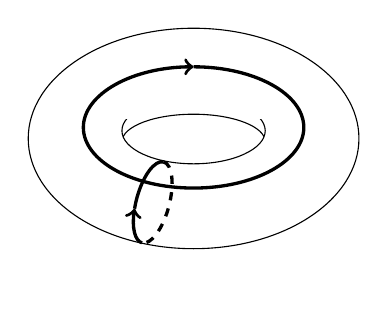
\begin{tikzpicture}[scale=1.4]
            \draw(0,1.5) ellipse (1.5 and 1);
            \begin{scope}
                \clip(0,1.57) ellipse (0.65 and 0.3);
                \draw(0,1.47) ellipse (0.65 and 0.25);
            \end{scope}
            \begin{scope}
                \clip(-1.5,0) rectangle (1.5,1.67);
                \draw(0,1.57) ellipse (0.65 and 0.3);
            \end{scope}
            \draw[very thick,shift={(0,2.15)},yscale=0.55,->] (0,0) arc (90:-270:1);
            \begin{scope}[shift={(-0.37,0.92)},rotate=-15,xscale=0.15,yscale=0.38]
                \draw[very thick,->] (0,-1) arc (-90:-165:1);
                \draw[very thick] ({-sin(75)},{-cos(75)}) arc (-165:-270:1);
                \draw[very thick,dashed] (0,1) arc (-270:-450:1);
            \end{scope}
        \end{tikzpicture}
    \end{figure}
    Choose coordinates \(0 \le \tilde{\phi}_i \le 2\pi\), \(1 \le i \le n\), such that each cycle can be written as
    \begin{equation}
        \Gamma_k = \{0 \le \tilde{\phi}_k \le 2\pi, \tilde{\phi_i} = \text{constant}, i \ne k\}.
    \end{equation}
    Define \(n\) action coordinates by
    \begin{equation}
        I_k = \frac{1}{2\pi}\oint_{\Gamma_k} \theta.
    \end{equation}
    Note that these don't depend on the choice of \(\Gamma_k\) (that is, up to homeomorphism). Thus \(I_k\) only depends on \(f_1,\dots,f_n\) and so are first integrals with \(H=f_1\).
    
    Choose a point \(q_0\) on \(\mathcal{M}_f\) and define a generating function 
    \begin{equation}
        S(q_j,I_j) = \int^q_{q_0}\theta.
    \end{equation}
    The angle coordinates are then defined by \(\phi_j = \pdv{S}{I_j}\).

    \((p_i,q_j) \to (I_i,\phi_j)\) is a canonical transformation, and we can write \(H=H(I_1,\dots,I_n)\).
\end{proof}

\begin{eg}
    All Hamiltonian systems in 2 dimensions are integrable. For example, take \(H(p,q) = \frac{1}{2}(p^2+\omega^2q^2)\) and \(\mathcal{M} = \RR^2\), \(\omega=\dd{p}\wedge\dd{q} = \dd{(p\dd{q})}\). Then \(\mathcal{M}_f = \{H(p,q) = E\}\), and we call \(E\) the energy. \(\mathcal{M}_f\) is an eclipse in the \(p\)-\(q\) plane; let \(\varepsilon\) be the region it encloses. We have action coordinate
    \begin{equation}
        I = \frac{1}{2\pi}\oint_{\mathcal{M}_f}p\dd{q} = \frac{1}{2\pi}\iint_{\epsilon}\dd{p}\dd{q} = \frac{\text{area}}{2\pi} = \frac{E}{\omega},
    \end{equation}
    so can write \(H(p,q) = E=\omega I\). On paths, \(I\) is constant, and we have \(\dot{\phi}(t) = \pdv{H}{I}=\omega\), so \(\phi(t) = \phi(0) + \omega t\).
\end{eg}

\section{Topological charges in field theory}
\lecture{11/02/16 \textbf{b}}
\subsection{Scalar kinks}

Consider Minkowski space \(\RR^{1,1}\) with metric \(\dd{s}^2 = \dd{t}^2 - \dd{x}^2\), and let \(\phi:\RR^{1,1}\to\RR\) be a scalar field with Lagrangian given by
\begin{equation}
    L = \int_\RR\frac{1}{2}\left(\phi_t^2-\phi_x^2-U(\phi)\right) \dd{x} = T - V.
\end{equation}
The Euler-Lagrange equations provide the equation of motion
\begin{equation}
    \phi_{tt} - \phi_{xx} = - \dv{U}{\phi}.
\end{equation}
We want the field to habe a stable ground state, so we need \(U(\phi)\ge U_0\) for some constant \(U_0\). We will normalise so that \(U_0=0\).

Now assume that \(U^{-1}(0) = \{\phi_1,\phi_2,\dots\}\) has more than one element.

\begin{figure}[H]
    \centering
    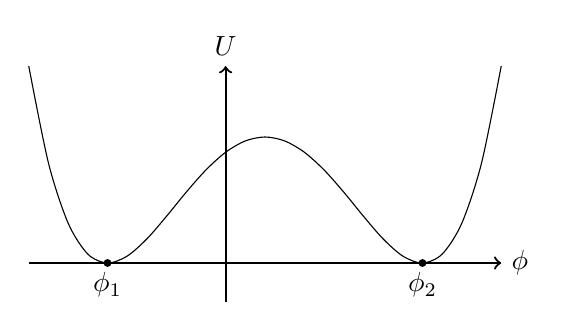
\begin{tikzpicture}
        \draw[domain=-3:3,smooth,variable=\x] plot ({\x},{(\x-2)*(\x-2)*(\x+2)*(\x+2)/10});
        \draw[thick,->] (-0.5,-0.5) -- (-0.5,2.5) node[above] {\(U\)};
        \draw[thick,->] (-3,0) -- (3,0) node[right] {\(\phi\)};
        \fill (-2,0) circle (0.05) node[below] {\(\phi_1\)};
        \fill (2,0) circle (0.05) node[below] {\(\phi_2\)};
    \end{tikzpicture}
\end{figure}

There are different ways in which we could handle this. One way is perturbation theory, leading to QFT, Feynman diagrams, and uncomfortable infinities. We choose a ground state, \(\phi_1\) say, and set \(\phi\approx\phi_1+\delta\phi\), where \(\delta\phi\) is small and dynamical. Then the Euler-Lagrange equations become \((\dalembertian + m^2)\delta\phi=0\).

Another way is to assume that finite energy solutions must approach an element of \(U^-1(0)\) sufficiently quickly as \(x\to\pm\infty\).

\begin{defn}
    \emph{Solitons} are non-singular, static, finite energy solutions to Euler-Lagrange equations.
\end{defn}

For example, we might have a soliton with \(\phi\to\phi_1\) as \(x\to-\infty\), and \(\phi\to\phi_2\) as \(x\to+\infty\) (called a \emph{non-perturbative kink}):

\begin{figure}[H]
    \centering
    \begin{tikzpicture}
        \draw[dashed,semithick] (-4,-1.3) -- (4,-1.3);
        \draw[dashed,semithick] (-4,1.3) -- (4,1.3);

        \node[fill=white,right] at (0,1.3) {\(\phi_2\)};
        \node[fill=white,right] at (0,-1.3) {\(\phi_1\)};

        \draw[thick,->] (0,-1.5) -- (0,1.5) node[above] {\(\phi\)};
        \draw[thick,->] (-4,0) -- (4,0) node[right] {\(x\)};

        \draw (4,1.25) .. controls (-1,1.15) and (-2,-1.2) .. (-4,-1.25);
    \end{tikzpicture}
\end{figure}

\begin{eg}
    Suppose \(U(\phi)=\frac{1}{2}\left[\dv{W(\phi)}{\phi}\right]^2\) (in such an instance \(W\) is called the \emph{superpotential}). The energy of the field is then given by 
    \begin{align}
        E &= \frac{1}{2} \int_\RR \dd{x} \Big(\phi_t^2+(\phi_x+W_\phi)^2 \mp 2 \underbrace{\phi_xW_\phi}_{=\dv{W}{x}}\Big) \\
          &= \frac{1}{2} \int_\RR \dd{x} \left(\phi_t^2 + (\phi_x \pm W_\phi)^2\right) \mp \left[W(\phi(\infty))-W(\phi(-\infty))\right] \\
          &\ge \left|W(\phi(\infty)) - W(\phi(-\infty))\right|.
    \end{align}
    This is the \emph{Bogomolny bound}, and it is saturated if the Bogomolny equations hold:
    \begin{equation}
        \phi_t=0,\quad \dv{\phi}{x} = \mp \dv{W}{\phi}
    \end{equation}
\end{eg}

\begin{defn}
    Let \(\phi_\pm = \lim_{x\to\pm\infty}\phi\). The \emph{topological charge} of \(\phi\) is given by
    \begin{equation}
        N = \phi_+ - \phi_- = \int_{-\infty}^{+\infty} \dv{\phi}{x} \dd{x}.
    \end{equation}
\end{defn}
The topological charge only depends on boundary conditions at \(\pm\infty\), and since \(E\) is finite, it is conserved. We can classify solitons by their topological charges:

\begin{figure}[H]
    \centering
    \subfloat[\(N>0\): kink]{
        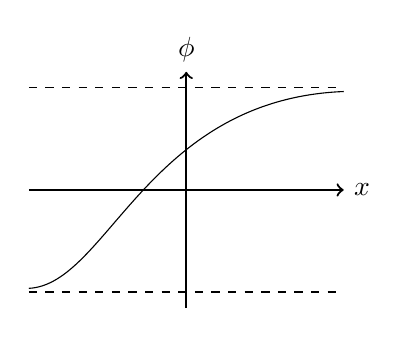
\begin{tikzpicture}[xscale=0.5]
            \draw[dashed,semithick] (-4,-1.3) -- (4,-1.3);
            \draw[dashed,semithick] (-4,1.3) -- (4,1.3);

            \draw[thick,->] (0,-1.5) -- (0,1.5) node[above] {\(\phi\)};
            \draw[thick,->] (-4,0) -- (4,0) node[right] {\(x\)};

            \draw (4,1.25) .. controls (-1,1.15) and (-2,-1.2) .. (-4,-1.25);
        \end{tikzpicture}
    }
    \subfloat[\(N<0\): antikink]{
        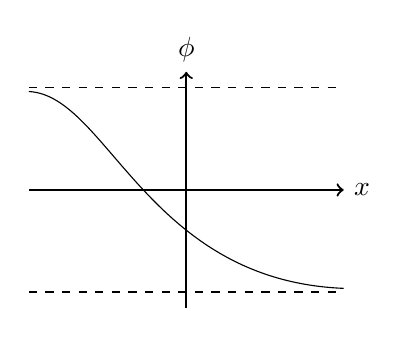
\begin{tikzpicture}[xscale=0.5]
            \draw[dashed,semithick] (-4,-1.3) -- (4,-1.3);
            \draw[dashed,semithick] (-4,1.3) -- (4,1.3);

            \draw[thick,->] (0,-1.5) -- (0,1.5) node[above] {\(\phi\)};
            \draw[thick,->] (-4,0) -- (4,0) node[right] {\(x\)};

            \draw (4,-1.25) .. controls (-1,-1.15) and (-2,1.2) .. (-4,1.25);
        \end{tikzpicture}
    }
    \subfloat[\(N=0\): trivial]{
        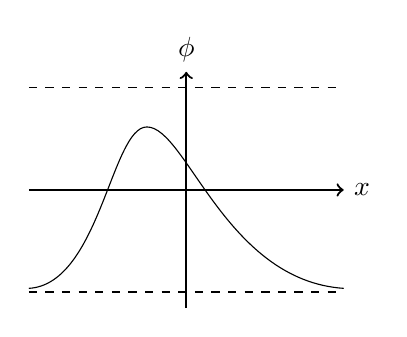
\begin{tikzpicture}[xscale=0.5]
            \draw[dashed,semithick] (-4,-1.3) -- (4,-1.3);
            \draw[dashed,semithick] (-4,1.3) -- (4,1.3);

            \draw[thick,->] (0,-1.5) -- (0,1.5) node[above] {\(\phi\)};
            \draw[thick,->] (-4,0) -- (4,0) node[right] {\(x\)};

            \draw (4,-1.25) .. controls (1,-1.15) and (0,0.8) .. (-1,0.8)
                .. controls (-1.9,0.8) and (-2.2,-1.2) .. (-4,-1.25);
        \end{tikzpicture}
    }
\end{figure}

\lecture{23/02/16}
\subsection{Degree of a map}
\begin{defn}
    Let \(\mathcal{M}\) and \(\mathcal{M}'\) be oriented, compact manifolds without boundary, and let \(f:\mathcal{M}\to\mathcal{M}'\) be a smooth map. The \emph{topological degree} of \(f\) is given by
    \begin{equation}
        \int_{\mathcal{M}}f^*(\operatorname{vol}(\mathcal{M}')) = \deg(f) \int_{\mathcal{M}'} \operatorname{vol}(\mathcal{M}'),
    \end{equation}
    where \(\omega = \operatorname{vol}(\mathcal{M}') \in \Lambda^n(\mathcal{M}')\) and \(\dim \mathcal{M} = \dim \mathcal{M}' = n\).
\end{defn}

Topological degree is independent of the choice of volume form \(\omega\). Suppose \(\omega\) and \(\hat{\omega}\) are such that
\begin{equation}
    \int_{\mathcal{M}'}\omega = \int_{\mathcal{M}'}\hat{\omega}.
\end{equation}
Then we have \(\int_{\mathcal{M}'}(\hat{\omega}-\omega)=0\), so \(\hat{\omega} = \omega+\dd{\alpha}\) for some \((n-1)\)-form \(\alpha\). Hence
\begin{equation}
    \int_{\mathcal{M}} f^*(\hat{\omega}) - \int_{\mathcal{M}} f^*(\omega)
    = \int_{\mathcal{M}} f^*(\dd{\alpha}) = \int_{\mathcal{M}} \dd{(f^*\alpha)}
    = \int_{\mathrlap{\partial\mathcal{M}=\varnothing}}\;\;f^*\alpha = 0
\end{equation}
Also, \(\deg(f) \in \ZZ\) and counts the number of pre-images of a point in \(\mathcal{M}'\) under \(f\).

\begin{theorem}
    \(\deg(f)\) is an integer given by 
    \begin{equation}
        \deg(f) = \sum_{\mathclap{x \in f^{-1}(y)}} \operatorname{sign}(J(x)),
    \end{equation}
    where \(J(x) = \det \left(\pdv{y^i}{x^j}\right)\), and \(y\) is regular.
\end{theorem}

\begin{eg}
    For functions \(f:S^1\to S^1\), \(\deg(f)\) is equivalent to the winding number.
    \begin{figure}[H]
        \centering
        \begin{tikzpicture}
            \clip (-1,-1) rectangle (10.5,7.5);
            \draw[semithick,dashed] (-1,3) -- (10,3);
            \draw[thick,->] (0,-1) -- (0,7) node[above] {\(f(\theta)\)};
            \draw[thick,->] (-1,0) -- (10,0) node[right] {\(\theta\)};
            \draw[semithick,dotted] (0,6) -- (9,6) -- (9,0);

            \node[above left] at (0,3) {\(f_0\)};
            \node[below left] at (0,0) {\(0\)};
            \node[below] at (9,0) {\(2\pi\)};
            \node[left] at (0,6) {\(2\pi\)};

            \draw (0,2) .. controls (1,6) and (2,-1) .. (4,6);
            \draw (4,0) .. controls (7,10) and (8,-2) .. (9,2);

            \node[below right] at (0.2,3) {\(+\)};
            \node[above right] at (1.2,3) {\(-\)};
            \node[below right] at (2.6,3) {\(+\)};
            \node[below right] at (5.0,3) {\(+\)};
            \node[above right] at (7.3,3) {\(-\)};
        \end{tikzpicture}
    \end{figure}
    We have
    \begin{equation}
        N = \sum_{\mathclap{\theta:f(\theta) = f_0}} \operatorname{sign}\left(\pdv{f}{\theta}\right),
    \end{equation}
    which is \(1-1+1+1-1=1\) in the above example.
    Equivalently we have
    \begin{equation}
        N = \frac{1}{\operatorname{vol}(S^1)}\int_{S^1} \dd{f} = \frac{1}{2\pi} \int^{2\pi}_0 \dv{f}{\theta}\dd{\theta}.
    \end{equation}
    For example, if we view \(S^1\) as the set of complex numbers with modulus \(1\), and let \(f(z)=z^k\), then \(\deg(f)=k\).
\end{eg}

\begin{eg}
    Consider \(f:S^2\to S^2\), and write \(f^a = f^a(x^i) \in \RR^3\), \(a=1,2,3\), \(|\vb{f}|=1\). Using spherical coordinates
    \begin{equation}
        x=r\sin\theta\cos\phi,\quad y=r\sin\theta\sin\phi,\quad z=r\cos\theta,
    \end{equation}
    it can be shown that
    \begin{equation}
        \deg(f) = \frac{1}{8\pi}\int\epsilon^{ij}\epsilon^{abc}f^a \pdv{f^b}{\rho^i} \pdv{f^c}{\rho^j}\dd[2]{\rho},
    \end{equation}
    where \(\rho^i = (\theta,\phi)\).
\end{eg}

\begin{eg}
    Let \(f:\mathcal{M}\to SU(2)\simeq S^3\), where \(\dim \mathcal{M}=3\). Then, using \(\operatorname{vol}(S^3) = 2\pi^2\), it can be shown that
    \begin{equation}
        \deg(f) = \frac{1}{24\pi^2}\int_{\mathcal{M}}\Tr\left[(f^-1\dd{f})^3\right].
    \end{equation}
\end{eg}

\subsection{Applications to physics}
\subsubsection*{Sigma model lumps}
Consider a field \(\phi:\RR^{2,1}\to S^{N-1}\subset\RR^N\) that is free (i.e.\ there is no potential, \(V(\phi)=0\)). The target space is non-linear. Treating \(\phi^a\) as a point in \(\RR^N\), the Lagrangian is
\begin{equation}
    \mathcal{L} = \frac{1}{2}\eta^{\mu\nu}\pdv{\phi^a}{x^\mu}\pdv{\phi^b}{x^\nu}\delta_{ab},
\end{equation}
and we have the added constraint
\begin{equation}
    \sum^N_{a=1} \phi^a \phi^a = 1.
\end{equation}
Thus we introduce a Lagrange multiplier, making the new Lagrangian
\begin{equation}
    \mathcal{L}'= \mathcal{L} - \frac{1}{2}\left(1-|\phi|^2\right).
\end{equation}
The Euler-Lagrange equations give \(\dalembertian\,\phi^a-\lambda\phi^a=0\). Dotting with \(\phi\), we find that \(\lambda = \sum_a\phi^a\dalembertian\,\phi^a\), so we obtain a non-linear set of field equations
\begin{equation}
    \dalembertian\,\phi^a - \left(\sum_{b=1}^N\phi^b\dalembertian\,\phi^b\right)\phi^a=0.
\end{equation}

Another way we could approach this would be to solve \(|\phi|^2=1\) for \(\phi^N\), and then substitute it back into the Lagrangian. We obtain
\begin{equation}
    \mathcal{L} = \frac{1}{2}g_{pq}(\phi)\eta_{\mu\nu}\pdv{\phi^p}{x^\mu}\pdv{\phi^q}{x^\nu} \qq{where}
    g_{pq} = \delta_{pq} + \frac{\phi^p\phi^q}{1-\sum_{r=1}^{N-1}\phi^r\phi^r},\quad
    p,q=1,\dots,N-1.
\end{equation}
\(g\) is the metric induced on \(S^{N-1}\) from \(\delta\) on \(\RR^N\). Proceeding with the Euler-Lagrange equations obtains the same equation as above.

In general a field \(\phi\) is a map between two pseudo-Riemannian manifolds, \((\Sigma,\eta)\stackrel{\phi}{\to}(\mathcal{M},g)\). Some examples:
\begin{itemize}
    \item For a point particle moving on a curved spacetime, we have \(\Sigma = \RR\), \(\eta=\dd{s}^2\) and \((\mathcal{M},g)\) is spacetime.
    \item In the bosonic sector of a superstring, \((\Sigma,g)\) is a Riemann surface (the string worldsheet), and \(\dim(\mathcal{M})=10\).
    \item When \(\dim(\Sigma) = k\), we say that we are considering a ``\((k-1)\)-brane''.
\end{itemize}

\lecture{25/02/16}
Return to the more specific case and set \(N=3\), so that \(\phi:\RR^{2,1}\to S^2\). For a static field, we have \(\phi:\RR^2\to S^2\). We want to consider finite energy conditions, i.e.\ those with finite
\begin{equation}
    E = \frac{1}{2}\int_{\RR^2}\partial_i\phi^a\partial_i\phi^a\dd{x}\dd{y}.
\end{equation}
If we change to polar coordinates, we see that (schematically) we then require \(|\nabla\phi|^2r\dd{r}\dd{\theta}\to0\) sufficiently quickly as \(r\to\infty\), or equivalently \(r|\nabla\phi^a|\to0\) as \(r\to\infty\). Thus we have \(\phi\to\phi^\infty\), a constant, at spatial infinity. Without loss of generality, we can take \(\phi^\infty\) to be the North pole, \((0,0,1)\). Since \(\phi\) is constant near spatial infinity, \(\phi\) extends to a one point compactification \(\RR^2+\{\infty\}=S^2\). 

Therefore static, finite energy configurations are maps \(\phi:S^2\to S^2\). These are classified by their degree (topological charge). This is only a partial classification, as fields can have different energies with the same \(\deg(\phi)\).

\begin{lemma}
    The energy is bounded from below, with \(E\ge 4\pi|\deg(\phi)|\). Equality is obtained when the 1st order Bogamolny equations hold:
    \begin{equation}
        \pdv{\phi^a}{x^i} = \pm\epsilon_{ij}\epsilon^{abc}\phi^b\pdv{\phi^c}{x^j}
    \end{equation}
\end{lemma}
\begin{proof}
    Consider the following inequality:
    \begin{equation}
        \int 
        \left( \partial_i\phi^a \pm \epsilon_{ij}\epsilon^{abc}\phi^b\partial_j\phi^c \right)
        \left( \partial_i\phi^a \pm \epsilon_{ik}\epsilon^{ade}\phi^d\partial_k\phi^e \right)
        \dd[2]{x} \ge 0
    \end{equation}
    If we use \(\epsilon_{ij}\epsilon_{ik} = \delta_{jk}\) and \(\epsilon^{abc}\epsilon^{ade}=\delta^{bd}\delta^{ce} - \delta^{be}\delta^{cd}\), and \(\phi^a\partial_i\phi^a = \frac{1}{2} \partial_i\phi^a\phi^a = 0\), then we see
    \begin{align}
        0 &\le \int\left[ \partial_i\phi^a\partial_i\phi^a + \delta_{jk}(\delta^{bd}\delta^{ce}-\delta^{be}\delta^{cd})\phi^b\phi^d\partial_j\phi^c\partial_k\phi^e \pm 2\epsilon_{ij}\partial_i\phi^a\epsilon^{abc}\phi^b\partial_j\phi^c\right] \dd[2]{x}\\
          & = 2E + 2E \pm 16\pi Q \ge 0,
    \end{align}
    where \(Q = \deg(\phi)\). Since \(E\ge0\), we obtain the result.
\end{proof}

\section{Gauge Theory}
\subsection{Hodge duality}
Consider \(\RR^n\), \(\eta=\dd{\vb{x}}^2-\dd{\vb{t}}^2\), with signature \((n-t,t)\), and \(x^a = (\vb{x},\vb{t})\), and assume we have a volume form \(\mathrm{vol} = \frac{1}{n!}\epsilon_{ab\dots c}\dd{x^a}\wedge\dd{x^b}\wedge\dots\wedge\dd{x^c}\). We have a natural inner product on \(p\)-forms given by
\begin{equation}
    (\alpha,\beta) = \frac{1}{p!} \alpha^{a_1\dots a_p}\beta_{a_1\dots a_p}.
\end{equation}
We define the Hodge operator \(*:\Lambda^p\to\Lambda^{n-p}\) by 
\begin{equation}
    \lambda\wedge\mu = (*\lambda,\mu)\cdot \mathrm{vol} \Forall \mu \in \Lambda^{n-p}.
\end{equation}
In components, we have
\begin{equation}
    (*\lambda)^{b_1\dots b_q} = \frac{(-1)^t}{p!}\epsilon{a_1\dots a_p b_1\dots b_q} \lambda_{a_1\dots a_p},
\end{equation}
and following things through, we find \(**\lambda = (-1)^{t+p(n-p)}\lambda\).

\begin{eg}
    Consider \(n=4,t=1,p=2\). Then \(**F=-F\) (e.g.\ the Maxwell field). We choose an orientation such that the volume form is \(\dd{x}\wedge\dd{y}\wedge\dd{z}\wedge\dd{t}\). With the Maxwell 2-form we usually write
    \begin{equation}
        F=-E_i\dd{t}\wedge\dd{x^i} + B_1\dd{x^2}\wedge\dd{x^3} + B_2\dd{x^3}\wedge\dd{x^1} + B_3 \dd{x^1}\wedge\dd{x^2}.
    \end{equation}
    Under the hodge star, we have \(*(\vb{E},\vb{B}) = (-\vb{B},\vb{E})\). Comparing with 
    \begin{equation}
        F=F_{0i}\dd{t}\wedge\dd{x^i} + \frac{1}{2}F_{ij}\dd{x^i}\wedge\dd{x^j},
    \end{equation}
    we see \(E_i = F_{0i}\) and \(B_i = \frac{1}{2}\epsilon_{ijk}F_{jk}\). The Maxwell equations \(\dd{F}=0\) give \(F=\dd{A}\) for some 1-form \(A\). If we write \(A = -\phi\dd{t} + A_i\dd{x^i}\), then we see
    \begin{equation}
        F=\dd{A} = \left(-\pdv{\phi}{x^i}-\pdv{A_i}{t}\right)\dd{x^i}\wedge\dd{t} + \partial_{[k}A_{i]}\dd{x^k}\wedge\dd{x^i},
    \end{equation}
    or
    \begin{equation}
        \vb{E} = -\dot{\vb{A}} - \nabla \phi,\quad \vb{B}=\nabla \times \vb{A}.
    \end{equation}
\end{eg}

\begin{eg}
    Consider \(n=4,t=0\) (Euclidean 4-space). For all 2-forms \(F\), we have \(**F=F\). If \(F=\dd{A}\) and \(*F=F\), then the Bianchi equations \(\dd{F}=0\) imply the Maxwell equations \(\dd{*F}=0\). The 2nd order Maxwell equations follow from the 1st order self-duality condition \(F=*F\).

    Note that any \(F\) can by written 
    \begin{equation}
        F = \underbrace{\frac{1}{2}(F+*F)}_{=F_+} + \underbrace{\frac{1}{2}(F-*F)}_{=F_-}.
    \end{equation}
    We have \(*F_+=F_+\) and \(*F_-=-F_-\), i.e.\ \(F_+\) is \emph{self-dual} and \(F_-\) is \emph{anti-self-dual}. In other words
    \begin{equation}
        \Lambda^2(\RR^4) = \Lambda^2_+ \oplus \Lambda^2_-,
    \end{equation}
    where the first vector space is dimension 6, and the latter two are dimension 3.
\end{eg}

\subsection{Yang-Mills equations}
Consider \((\RR^n,\eta,\mathrm{vol})\), and \(G\) a Lie group with Lie algebra \(\mathfrak{g}\). A gauge potential \(A\) is a \(\mathfrak{G}\)-valued 1-form on \(\RR^n\). Expanding in components, we write
\begin{equation}
    A = A_b\dd{x^b} = A^\alpha_b T_\alpha \dd{x^b},\quad A^\alpha_b:\RR^n\to\RR,
\end{equation}
where \(T_\alpha\), \(\alpha=1,\dots,\dim G\) is a basis of \(\mathfrak{g}\), with structure constants given by \([T_\alpha,T_\beta] = c_{\alpha\beta\psi}T_\gamma\). The gauge field corresponding to \(A\) is
\begin{equation}
    F = \dd{A} + A\wedge A = \frac{1}{2} F_{ab} \dd{x^a}\wedge\dd{x^b}.
\end{equation}
Evaluating the components of \(F\), we have
\begin{equation}
    F_{ab} = \partial_a A_b - \partial_b A_a + [A_a,A_b] = [\Dd{}_a,\Dd{}_b],
\end{equation}
where \(\Dd{}=\dd{} + A\) is the covariant derivative of \(A\). 

We identify \((A,A')\) and \((F,F')\) if
\begin{equation}
    A' = gAg^{-1} - \dd{g}\cdot g^{-1},\quad F' = gFg^{-1}
\end{equation}
for some \(g:\RR^n\to G\), called a gauge transformation.

\(F\) is in the adjoint representation, so we can deduce the Bianchi identity
\begin{align}
    \Dd{F} &= \dd{F} + [A,F] \\
           &= \dd[2]{A} + \dd{A}\wedge A - A \wedge \dd{A} + A\wedge\dd{A} - \dd{A}\wedge A + A \wedge A \wedge A - A \wedge A \wedge A \\
           &= 0.
\end{align}

The Yang-Mills equations are \(\Dd{*F} = 0\). These arise from the action
\begin{equation}
    S = -\int \Tr(F\wedge *F).
\end{equation}
If we set \(G=U(1)\), we recover Maxwell theory. If we take \(G=SU(2)\), then \(\mathcal{g}\) is the set of \(2\times 2\) anti-Hermitian matrices, and we have a basis where \([T_\alpha,T_\beta] = -\epsilon_{\alpha\beta\gamma}T_\gamma\). In this basis, \(\Tr(T_\alpha T_\beta) = -\frac{1}{2}\delta_{\alpha\beta}\), and hence
\begin{equation}
    -\Tr(F\wedge *F) = -\frac{1}{2}\Tr(F^{ab}F_{ab})\mathrm{vol}.
\end{equation}

\subsection{Yang-Mills instantons and Chern forms}
\begin{defn}
    \emph{Instantons} are non-singular equations of motion in Euclidean space (\(\RR^4\)), whose action is finite.
\end{defn}

\lecture{01/03/16}
Consider \(\RR^4\), \(\eta=\delta\), with boundary conditions on \(A\) such that
\begin{equation}
    F_{ab}(x) \sim O\left(\frac{1}{r^3}\right),\quad
    A_a(x) \sim O\left(\frac{1}{r^2}\right) - \partial_a g \cdot g^{-1}
\end{equation}
as \(r \to \infty\). The gauge transformation \(g\) need only be defined asymptotically as \(r \to \infty\) on \(\partial\RR^4\simeq S^3_\infty\), so for example \(g:S^3_\infty \to G = SU(2)=S^3\). The topological degree of \(g\) will become relevant.

Consider gauge theories on \(\RR^n\) for general \(n\). We define the Chern forms in the following way. Let
\begin{equation}
    C(F) = \det \left(\identity + \frac{i}{2\pi}F\right) = 1 + C_1(F) + C_2(F) + \dots.
\end{equation}
\(C_p(F)\) is the \(2p\)-form part of the Chern form and is \(O(F^p)\); it is called the \emph{\(p^\text{th}\) Chern form}. \(C\) is gauge invariant (\(C(F) = C(gFg^{-1})\)), and closed (by the Bianchi identity).

We have:
\begin{itemize}
    \item \(C_1(F) = \frac{i}{2\pi}\Tr(F)\). This vanishes for \(G=SU(2)\) (but not \(G=U(1)\)).
    \item \(C_2(F) = \frac{1}{8\pi^2}\left(\Tr(F\wedge F) - \Tr F\wedge \Tr F\right)\). For \(G=SU(2)\), this is \(C_2(F) = \frac{1}{8\pi^2}\Tr(F\wedge F)\).
\end{itemize}
Using the Bianchi identity \(\Dd{F} = \dd{f} + A\wedge F - F\wedge A = 0\), we have
\begin{equation}
    \dd{C_2} = \frac{1}{4\pi^2}\Tr(\dd{F}\wedge F) = \frac{1}{4\pi^2}\Tr(-A\wedge F \wedge F + F \wedge A \wedge F) = 0.
\end{equation}
Hence \(C_2\) is exact, so we can write \(C_2 = \dd{Y_3}\), where \(Y_3\) is the \emph{Chern-Simons 3-form}. It is an exercise to verify that
\begin{equation}
    Y_3 = \frac{1}{8\pi^2}\Tr(\dd{A}\wedge A + \frac{2}{3}A^3).
\end{equation}

Returning to \(n-4\), we define the \emph{Chern number} by
\begin{equation}
    c_2 = \int_{\RR^4} C_2(F).
\end{equation}

We have
\begin{align}
    c_2 &= \int_{\RR^4} \dd{Y_3} \\
        &= \frac{1}{8\pi^2} \int_{\RR^4} \dd{\left[\Tr\left(F\wedge A - \frac{1}{3}A^3\right)\right]} \\
        &= - \frac{1}{24\pi^2} \int_{S^3_\infty} \Tr(A^3) \\
        &= \frac{1}{24\pi^2} \int_{S^3} \Tr\left[(\dd{g}\cdot g^{-1})^3\right] \\
        &= \deg(g) \in \ZZ.
\end{align}
This integer gives a classification of instantons on \(\RR^4\).

\begin{theorem}
    The Yang-Mills action \(S = -\int_{\RR^4} \Tr(F\wedge * F)\) on a given topological sector \(c_2\ge0\) is bounded from below by \(8\pi^2c_2\). The bound is saturated iff the anti-self-dual (ASD) Yang-Mills equations hold (\(F=-*F\), or \(F_{12} = -F_{34}\), \(F_{13} = -F_{42}\), \(F_{14}=-F_{23}\)).
\end{theorem}
\begin{proof}
    First note that \(F\wedge F = *F\wedge*F\) for any 2-form \(F\) (this can be seen as the difference of two squares). Thus we have
    \begin{equation}
        S = -\frac{1}{2}\underbrace{\int_{\RR^4}\Tr\left[(F+*F)\wedge(F+*F)\right]}_{\text{total square, trace negative definite}} + \underbrace{\int_{\RR^4}\Tr(F\wedge F)}_{=8\pi^2c_2} \ge 8\pi^2c_2,
    \end{equation}
    and equality iff \(F+*F=0\).
\end{proof}
This is the Bogomolny bound for the Yang-Mills actions. A similar calculation with \(c_2 \le 0\) gives SDYM (\(F=*F\)). 

If \(*F=\pm F\), then \(\Dd{*F}=\pm \Dd{F} = 0\), so the full Yang-Mills equations hold.

The \emph{instanton number} is \(k=-c_2\).

\subsection{Fibre bundles \& connections}
\lecture{03/03/16}
Yang-Mills theory is equivalent to a theory of connections on principal bundles, with the gauge group \(G\) on fibres. Fibre bundles are ``locally product manifolds''. For example, the cylinder and M\"obius band are both examples of \(S^1\) ``locally multiplied'' by \(\RR\). More concretely:
\begin{defn}
    A \emph{fibre bundle} \(\{E,\pi,B,F,G\}\) is a structure consisting of:
    \begin{enumerate}
        \item Two manifolds \(E\) and \(B\) with \(\dim E>\dim B\), and a smooth map \(\pi:E\to B\). \(\pi\) is the \emph{projection} from the \emph{total space} \(E\) onto the \emph{base} \(B\).
        \item A manifold \(F\) (the \emph{fibre}) such that for any point \(x\in B\), there exists an open \(U_\alpha\subset B\) with \(x \in U_\alpha\) and an diffeomorphism \(\phi_\alpha:U_\alpha\times F\to \pi^{-1}(U_\alpha)\) satisfying \(\pi(\phi_\alpha(x,f)) = x\).
        \item Transition functions \(\phi_{\alpha\beta}=\phi_\alpha^{-1}\circ\phi_\beta\) and \(G \ni \phi_{\alpha\beta}:F\to F\), \(f\mapsto\phi_{\alpha\beta}(x,f)\) with \(x\in U_\alpha\cap U_\beta\). \(G\) is a Lie group: the \emph{structure group} of the bundle, the group of transformations of \(F\). We require \(\phi_{\alpha\alpha} = \) identity, and \(\phi_{\alpha\beta}\phi_{\beta\gamma} = \phi_{\alpha\gamma}\) for \(x \in U_\alpha\cap U_\beta\cap U_\gamma\) (this is the ``cocycle relation'').
    \end{enumerate}
\end{defn}

A \emph{principal bundle} has \(F=G\), and \(G\) acts on \(F\) by left translations.

A \emph{vector bundle} has \(F=\RR^n\) and \(G \subset GL(n,\RR)\).

A \emph{trivial bundle} has \(E\simeq B \times F\). It turns out that a bundle is always trivial if \(B\) is contractible.

\begin{eg}
    \(E=TB=\bigcup_{x\in B} T_x B\), the tangent bundle, is a vector bundle with \(F_x = \pi^{-1}(x) \simeq \RR^n\) and \(G = GL(n,\RR)\). Points in \(E\) take the form \((\vb{x},\vb{v})\), where \(\vb{x}\) is a ``position'', and \(\vb{v}\) is a ``velocity''.
\end{eg}

\begin{eg}
    Consider \(B=S^2\), \(F=G=U(1)\simeq S^1\). This is the ``magnetic monopole bundle''.
    \begin{figure}[H]
        \centering
        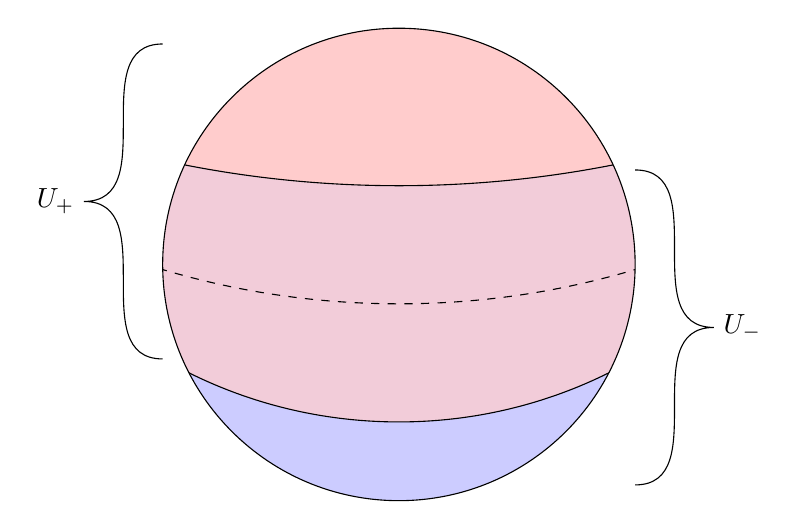
\begin{tikzpicture}
            \fill[blue!20] (0,0) circle (3);
            \begin{scope}
                \clip (0,0) circle (3);
                \fill[purple!20] (0,4) circle (6);
                \fill[red!20] (0,15) circle (14);

                \draw[dashed] (0,10) circle (10.5);
                \draw (0,4) circle (6);
                \draw (0,15) circle (14);
            \end{scope}
            \draw (0,0) circle (3);

            \draw[rotate=180] (-3,2.8) .. controls (-4,2.8) and (-3,0.8) .. (-4,0.8)
                node[right] {\(U_-\)}
                .. controls (-3,0.8) and (-4,-1.2) .. (-3,-1.2);
            \draw (-3,2.8) .. controls (-4,2.8) and (-3,0.8) .. (-4,0.8)
                node[left] {\(U_+\)}
                .. controls (-3,0.8) and (-4,-1.2) .. (-3,-1.2);
        \end{tikzpicture}
    \end{figure}
    We can write \(B=U_+ \cup U_-\) as shown in the diagram. We use a fibre coordinate \(\psi\) for \(e^{i\psi}\in U(1)\), with \(0\le\psi\le2\pi\). On the base we have local spherical coordinates \((\theta,\phi)\) with \(0\le\theta\le\pi\) and \(0\le\phi\le2\pi\).
    Suppose a point in \(U_+\cap U_-\) has coordinates \((\theta,\phi,e^{i\psi_+})\) on \(U_+\times U(1)\) and coordinates \((\theta,\phi,e^{i\psi_-})\) on \(U_-\times U(1)\). We have \(e^{i\psi_-} = e^{in\phi}e^{i\psi_+}\). In order for \(E\) to be a manifold \(n\) must be an integer, and it is known as the \emph{monopole number}. \(n\) classifies the \(U(1)\) principal bundles over \(S^2\). If \(n=0\), then \(E=S^2\times S^1\), a trivial bundle. If \(n=1\) then \(E=S^3\), and this is known as the Hopf fibration.
\end{eg}

\lecture{08/03/16}

\begin{eg}
    Consider bundles with \(B=S^2\), \(F=G=S^1\), and monopole number \(n=1\), so \(E=S^3\). We can view \(S^3\) as a subset of \(\CC^2\) with
    \begin{equation}
        S^3 = \{(z_1,z_2)\in \CC^2 \st |z_1|^2 + |z_2|^2\}.
    \end{equation}
    \(U(1)\) acts on \(S^3\) by right multiplication \((z_1,z_2) \to (z_1e^{i\alpha},z_2e^{i\alpha})\). Note that this action preserves the ratio \(z_1/z_2 \in S^2\), so \(\pi:S^3\to S^2=S^3/U(1)\).

    Another description involves taking \(\CC^2\simeq\RR^4\). A complex line \(A_1z_1 + A_2z_2=0\) through the origin is \(\CC\mathbb{P}^1 \simeq S^1\), and this intersects \(S^3\) in \(S^1\). This is a fibre over a point \(z_1/z_2 \in \mathbb{CP}^1\simeq S^2\).
\end{eg}

\begin{defn}
    A section of a bundle \(\pi:E\to B\) is a map \(s:B\to E\) such that \(\pi\circ s = \) identity on \(B\). This generalises functions on \(B\).
\end{defn}

\begin{eg}
    Vector fields are sections of the tangent bundle \(TB\), \(x^a \in B \to V^b(x^a)\pdv{x^b}\).
\end{eg}

\begin{lemma}
    A principal bundle admits a global section iff it is trivial.
\end{lemma}
\begin{proof}
    Let \(x\in B\). Suppose \(s:B\to E\) is such a section. Then for all \(p \in \pi^{-1}(x)= G_x\), we can write \(p=s(x)\cdot R_g(p)\), where \(R_g(p)\) is the right translation of \(G\) on \(G_x\) moving \(s(x)\) to \(p\). Then \(E\to(x\ne\pi(p),g(p)\in B\times G\) is a global trivialisation.
\end{proof}

\begin{defn}
    A \emph{connection} on a principal bundle \((E,\pi,B,G)\) is a \(\mathfrak{g}\)-valued 1-form whose vertical component (i.e.\ the part cotangent to \(G\)) is the Maurer-Cartan form on \(G\).
\end{defn}

In local coordinates we can write a connection as \(\omega=\gamma^{-1}A\gamma + \gamma^{-1}\dd{\gamma}\), where \(A\) is a \(\mathfrak{g}\)-valued 1-form on \(B\), \(\gamma\in G\) are fibre coordinates, and \(\gamma^{-1}\dd{\gamma}\) is the Maurer-Cartan 1-form.

Let \(U,U'\) be two overlapping open sets on \(B\), and \(g=g_{UU'}\) be the transition function on \(B\) defining \(E\), so that \(\gamma' = g\gamma\). We want \(A'\) such that
\begin{equation}
    \omega = \begin{Bmatrix}
        \gamma^{-1}A\gamma + \gamma^{-1}\dd{\gamma} &\text{on}& U\times G \\
        {\gamma'}^{-1}A'\gamma' + {\gamma'}^{-1}\dd{\gamma'} &\text{on}& U'\times G
    \end{Bmatrix}\, \text{are equal on \(U\cap U'\)}.
\end{equation}
From this, we obtain
\begin{equation}
    A' = gAg^{-1} - \dd{g}\cdot g^{-1},
\end{equation}
so \(A\) and \(A'\) are related by a gauge transformation on \(B\).

\begin{defn}
    The \emph{curvature} is a \(\mathfrak{g}\)-valued 2-form on \(E\) defined as
    \begin{equation}
        \Omega = \dd{\omega} + \omega\wedge\omega.
    \end{equation}
\end{defn}

Using the form of \(\omega\) above, we have
\begin{align}
    \Omega &= \dd{\gamma^{-1}A\gamma + \gamma^{-1}\dd{\gamma}} + \gamma^{-1}A\wedge A\gamma + \gamma^{-1} A \dd{\gamma} + \underbrace{\gamma^{-1}\dd{\gamma}\gamma^{-1}}_{=-\dd{(\gamma^{-1})}}\wedge A\gamma \\
           &= \gamma^{-1}(\dd{A} + A\wedge A) \gamma\\
           &= \gamma^{-1} F \gamma.
\end{align}

Any local section \(\gamma:B\to G\) can be used to pull back \((\omega,\Omega)\) from \(E\) to \(B\) such that \(A = \gamma^*(\omega)\) is the gauge potential, and \(F=\gamma^*(\Omega)\) is the gauge field. Gauge transformations on \(B\) are then just equivalent to a change of sections.

If \(E\to B\) is non-trivial, then a global section does not exist, and \(A\) can only be defined locally on \(B\).

\lecture{10/03/16}
\subsubsection*{Horizontal decomposition}
Let \((E,B,\pi,G)\) be a principal bundle. Given a connection \(\omega\) on that bundle, we can define a splitting \(TE = H(E)\oplus V(E)\) in the following way.
\begin{defn}
    The \emph{horizontal subbundle} is
    \begin{equation}
        H(P) = \{X\in TE \st X\contract\,\omega=0\}.
    \end{equation}
\end{defn}
Horizontal vectors \(X\) annihilate \(\omega = \gamma^{-1}A\gamma + \gamma^{-1}\dd{\gamma}\), so they also annihilate \(\gamma\omega\gamma^{-1}=A + \dd{\gamma}\cdot\gamma^{-1}\). We write \(\dd{\gamma}\cdot\gamma^{-1}=\lambda^\alpha\otimes T_\alpha\), where \(T_\alpha\) is a basis of \(\mathfrak{g}\) with structure constants given by \([T_\alpha,T_\beta] = f_{\alpha\beta}^\gamma T_\gamma\).

We claim that a basis of \(H(E)\) is \(D_a=\pdv{x^a} - A_a^\alpha R_\alpha\), where \(R_\alpha\) are right-invariant vector fields on \(G\). As a check, we have
\begin{equation}
    D_a\contract(\gamma\omega\gamma^{-1}) = \left(\pdv{x^a} - A_a^\alpha R_\alpha\right)\contract(A_b\dd{x^b} + \lambda^\beta\otimes T_\beta) = A_a - A^\alpha_a T_\alpha = 0.
\end{equation}

Frobenius integrability of \(H(E)\) requires \([H(E),H(E)]\subset H(E)\), so we see that curvature is an obstruction to this, since
\begin{equation}
    [D_a,D_b] = -F_{ab}^\alpha R_\alpha \qq{where} F_{ab}=\partial_a A_b - \partial_b A_a + [A_a,A_b],
\end{equation}
and this only belongs to \(H(E)\) if \(F=0\).

\subsection{Back to Yang-Mills instantons}
For any instanton on \(\RR^4\), there exists a bundle \(E\) over \(S^4\) which (under stereographic projection \(S^4\to\RR^4\)) maps a pullback of a connection to Yang-Mills potentials. Boundary conditions on \(\RR^4\) are equivalent to an extension of the instanton to \(S^4\).

We cover \(S^4\) by two regions \(U_\pm\) such that \(U_+\cap U_-=S^3\times[-\epsilon,\epsilon]\) for some \(\epsilon\). Consider \(E\to S^4\), \(G=SU(2)\), with a connection
\begin{equation}
    \omega = 
    \begin{cases}
        \gamma_+^{-1}A_+\gamma_+ + \gamma_+^{-1}\dd{\gamma_+} & \text{on \(U_+\)}, \\
        \gamma_-^{-1}A_-\gamma_+ + \gamma_-^{-1}\dd{\gamma_-} & \text{on \(U_-\)}. 
    \end{cases}
\end{equation}
On \(U_+\cap U_-\), \(\gamma_- = g\gamma_+\) for some \(g:U_+\cap U_- \to SU(2)\). The curvature is
\begin{equation}
    \Omega = \dd{\omega} + \omega \wedge\omega = 
    \begin{cases}
        \gamma_+^{-1}F_+\gamma_+ & \text{on \(U_+\)}, \\
        \gamma_-^{-1}F_-\gamma_- & \text{on \(U_-\)}.
    \end{cases}
\end{equation}

Introduce Chern-Simons 3-forms \(Y_\pm\) on \(U_\pm\). Then we have
\begin{align}
    k &= -\frac{1}{8\pi^2} \int_{S^4} \Tr(\Omega \wedge \Omega) \\
      &= -\frac{1}{8\pi^2} \left[ \int_{U_+} \Tr(F_+\wedge F_+) + \int_{U_-} \Tr(F_-\wedge F_-) \right] \quad \text{in the limit \(\epsilon \to 0\)} \\
      &= -\frac{1}{8\pi^2} \int_{S^3} \left[\Tr\left(F_+\wedge A_+ - \frac{1}{3}A_+^3\right) - \Tr\left(F_-\wedge A_- - \frac{1}{3}A_-^3\right) \right] \\
    \intertext{(now use the gauge equivalence of \(A_+\) and \(A_-\))}
    &= -\frac{1}{8\pi^2}\int_{S^3} \Tr\left(\frac{1}{3}(\dd{g}\cdot g^{-1})^3\right) - \underbrace{\dd{\left[(A_+\wedge\dd{g})\cdot g^{-1}\right]}}_{\mathclap{\text{vanishes in integral since \(\partial S^3 = \varnothing\)}}} \\
    &= -\frac{1}{24\pi^2} \int_{S^3} \Tr \left((\dd{g}\cdot g^{-1})^3\right) \in \ZZ.
\end{align}
This is the same formula as before, but we have a different interpretation. \(g\) is a transition function for \(E\to S^4\).

All information about instantons is in these topological numbers; they are connection invariant.

\end{document}
